% Sample Dissertation, Thesis, or Document %
%            for use with the              %
%  University of Arizona Thesis Class,     %
%               uathesis.cls               %
%------------------------------------------%

% We'll use the uathesis document class (duh).  The uncommented line
% below will produce a Dissertation, the others would produce a Thesis
% or a Document.  There are other options available to you like turning
% on the copyright statement and replacing the year on the title page
% with a "generated on" stamp (handy for early drafts).  To find out
% what the available options are, take a look into the uathesis.cls
% file and look for the \DeclareOption commands near the top of that
% file.
% There are five copyright options.  Copyright, no copyright, and three
% different Creative Commons licences.  Use the one you want (If you go
% Creative Commons, I (DM) think the CC-BY-ND makes the most sense)  See
% uathesis.cls for the reason why the non-commercial licenses are not
% included.
%\documentclass[dissertation]{uathesis}
%\documentclass[dissertation,copyright]{uathesis}
%\documentclass[dissertation,CC-BY]{uathesis}
%\documentclass[dissertation,CC-BY-SA]{uathesis}
\documentclass[dissertation,CC-BY-ND]{uathesis}
%\documentclass[dissertation,generatedon]{uathesis}
%\documentclass[thesis]{uathesis}
%\documentclass[document]{uathesis}

% Package Usage
% These are the packages that we need
%\usepackage{algorithm}
%\usepackage{algorithmic}
%\usepackage[ruled,boxed,noend]{algorithm2e}
\usepackage{graphicx}
\usepackage{natbib}			% natbib is available on most systems, and is
					% terribly handy.
					% If you want to use a different Bibliography package, 
					% you should be able to, just change this
					% and the \bibliographystyle command below.  Be warned
					% that you may need to do a little hacking to get
					% the REFERENCES item to show up in your TOC.
\usepackage{latexsym}

\usepackage{algorithm}
\usepackage{algorithmic}
\usepackage{fancyvrb, fancyhdr, theorem, latexsym, color, longtable}
\definecolor{common}{rgb}{0.13, 0.67, 0.8}
\definecolor{omit}{rgb}{1.0, 0.25, 0.25}
\definecolor{orange}{rgb}{0.93, 0.53, 0.18}

\usepackage{multirow}
\usepackage{url}
\usepackage{bm}
\usepackage{fixltx2e}
\usepackage{tabularx}
\usepackage{comment}
\usepackage{amsmath,amssymb}
%\usepackage{verbatim}
%\usepackage{caption}
%\usepackage{subcaption}
%\usepackage{fixltx2e}
%\usepackage{float}
\usepackage{supertabular,booktabs}
%\usepackage{enumerate}
%\usepackage{afterpage}
%\usepackage{array}
%%\usepackage{setspace}


% Compatibility with the AASTEX package 
% of the American Astronomical Society.
%\usepackage{deluxetable}		% Allows use of AASTEX deluxe tables
%\usepackage{aastex_hack}		% Allows other AASTEX functionality.

% These are other packages that you might find useful.
% For controlling the fonts, see
% http://www.math.uiuc.edu/~hartke/computer/latex/survey/survey.html
% The following is a nice font set:
%\usepackage{mathtime}			% Times for letters; Belleek math.
%
%\usepackage{amsmath}			% AMS Math (advanced math typesetting)
%\usepackage{lscape}			% Used for making fitting large tables in by putting them landscape
%\usepackage{refs}			
%
% If you are using hyper-ref (recommended), this command must go after all 
% other package inclusions (from the hyperref package documentation).
% The purpose of hyperref is to make the PDF created extensively
% cross-referenced.
\usepackage[bookmarks,colorlinks=true,urlcolor=black,linkcolor=black,citecolor=black]{hyperref}

\newcommand{\todo}[1]{\textcolor{red}{TODO: #1}}
\newcommand{\remove}[1]{\textcolor{omit}{OMIT?: #1}}
\newcommand{\address}[1]{\textcolor{blue}{-- #1}}
\newcommand{\note}[1]{\textcolor{red}{#1}}
\newcommand{\svmr}{{SVM$^{rank}$}}
\newcommand{\code}[1]{{\tt {\small #1}}}
\newcommand{\qn}{{{\bf Q}$^\textbf{{\small N}}$}}
\newcommand{\ssa}{{{\scriptsize $^{*}$}}}

\DeclareMathOperator*{\argmax}{arg\,max}

% Set up some values.
\completetitle{Computational Natural Language Inference: Robust and Interpretable Question Answering}
\fullname{Rebecca Reynolds Sharp} % Grad college wants your full name here.
\degreename{Doctor of Philosophy}	% Title of your degree.

\begin{document}

% Set up the title page
\maketitlepage
{DEPARTMENT OF LINGUISTICS}	% Title of your department.
{2017}							

% Insert the approval form.  Note that for electronic submission
% of your Ph. D. dissertation, you must bring *two* copies of the
% approval page to your final defense.  These must be signed by
% the committee.  Make two photocopies: one for Pam and the other
% for your records.  Then, bring the two signed originals to the
% graduate college when you submit the final version of the
% dissertation to the University of Arizona.
%\approval
%{\textcolor{red}{11} August 2017}		% Defense Date	
%{Michael Hammond}		% Dissertation Director
%{Mihai Surdeanu}		% 2nd committee member
%{Michael Hammond}		% 1st committee member
%{Mihai Surdeanu}		% 2nd committee member
%{Peter Jansen}		    % 3rd committee member
%{} % 4th committee member (leave empty if None)

% Include the ``Statement by Author'' for Dissertations
%\statementbyauthor

% bs: Doesn't apply to me I think:
% If this is a Thesis, use the following form, with your thesis director's
% name and title in the square brackets like so (you should also omit the 
% approval form insertion above):
%\statementbyauthor[Jane M. Doe\\Professor of Chemistry]

%% Include the ``Acknowledgements''
%\incacknowledgements{acknowledgements}
%
%% Include the ``Dedication''
%\incdedication{dedication}
%
%% Create a ``Table of Contents''
\tableofcontents
%
%% Create a ``List of Figures''
%\listoffigures
%
%% Create a ``List of Tables''
%\listoftables
%
%% Include the ``Abstract''
%\incabstract{abstract}

% Include the various chapters
\chapter{INTRODUCTION\label{chapter:introduction}}

text

\section{Overview\label{sec:overview}}

Some text/outline of the body of the document.
\chapter{RELATED WORK\label{chapter:related_work}}

In one sense, QA systems can be described in terms of their position along a formality continuum ranging from shallow models that rely on information retrieval, lexical semantics, or alignment, to highly structured models based on first order logic (FOL).

On the shallower end of the spectrum,  QA models can be constructed either from structured text, such as question--answer pairs, or unstructured text.  Alignment models~\citep{Berger:00,echihabi2003noisy,Soricut:06,Riezler:etal:2007,Surdeanu:11,yao2013}  require aligned question--answer pairs for training, a burden which often limits their practical usage.  In Chapter \ref{chapter:naacl2015} we address this burden by proposing a method for using the discourse structure of free text as a surrogate for this alignment structure. \todo{ref to a related work section in that chapter? or keep it here in a subsection?}

Lexical semantic models such as neural-network language models~\citep{jansen14,sultan-etal:2014:TACL,yih13}, on the other hand, have the advantage of being readily constructed from free text.  
\citet{fried2015higher} called these approaches first-order models because associations are explicitly learned, and introduced a higher-order lexical semantics QA model where indirect associations are detected through traversals of the association graph.  
Other recent efforts have applied deep learning architectures to QA to learn non-linear answer scoring functions that model lexical semantics~\citep{Iyyer2014,nips15_hermann}.

These alignment and lexical semantic approaches, however do not take into account the wide variety of question type which often exist in any given question set, and therefore attempt to answer \emph{all} questions with the same set of word association values.  To address this, we propose an approach in Chapter \ref{chapter:emnlp2016} for training a dedicated set of word embeddings that are customized to a particular semantic relation (here, causality) and demonstrate that the semantic information contained in the embeddings is complementary to that which is contained in standard word embeddings and useful in a causal QA task.

While these word association approaches to QA have shown robust performance across a variety of tasks, one continuing disadvantage of these methods is that, even when a correct answer is selected, there is no clear human-readable justification for that selection.  This limits our ability to effectively understand model performance and adjust for errors accordingly.

Closer to the other end of the formality continuum, several approaches were proposed to not only select a correct answer, but also provide a formally valid justification for that answer.  For example, some QA systems have sought to answer questions by creating formal proofs driven by logic reasoning~\citep{moldovan2003cogex,moldovan2007cogex,balduccini2008knowledge,maccartney2009natural,liang2013learning,lewis2013combining}, answer-set programming \citep{baral2006using,baral2011towards,baral2012answering,baral2012knowledge}, or connecting semantic graphs~\citep{banarescu2012amr,sharmatowards}. 
However, the formal representations used in these systems, e.g., logic forms, are both expensive to generate and tend to be brittle because they rely extensively on imperfect tools for unsolved problems such as complete syntactic analysis and word sense disambiguation.

In Chapter \ref{chapter:cl2017}, we offer a lightly-structured sentence representation generated by our approach (see Section \ref{sec-cl2017:tag}) as a shallower and consequently more robust approximation of those logical forms, and show that they are well-suited for the complex questions (see Section \ref{sec:mcqa} for more details) we tackle.
This approach allows us to robustly aggregate information from a variety of knowledge sources to create human-readable answer justifications.  
It is these justifications which are then ranked in order to choose the correct answer, using a reranking perceptron with a latent layer that models the correctness of those justifications.

While this approach is shallower than many of the approaches based on formal representations, it still requires decomposing free text resources into lightly-structured representations and performing a fairly expensive aggregation.  In practice, this limits its use with very large text corpora.  Additionally, the perceptron-based learning framework is inherently limited by its assumption of linearlly-separable data.  To address these, in Chapter \ref{chapter:emnlp2017} we propose a shallower version of this model that can learn an embedded representation of the question, answer, and candidate justification texts and that can re-rank justifications using these representations alongside a small set of explicit features.  

In both of these latter approaches, the way we have formulated our justification selection (as a re-ranking of knowledge base sentences) is related to, but yet distinct from the task of answer sentence selection \cite[][inter alia]{Wang2010ProbabilisticTM, Severyn:12,Severyn:13a,Severyn:13b,Severyn2015LearningTR,wang2015long}.  Answer sentence selection is typically framed as a fully or semi-supervised task for factoid questions, where a correctly selected sentence fully contains the answer text.
Here, we have a variety of questions, many of which are non-factoid.  Additionally, we have no direct supervision for our justification selection (i.e., no labels as to which sentences are good justifications for our answers), motivating our distant supervision approach where the performance on our QA task serves as supervision for selecting good justifications.  Further, we are not actually looking for sentences that \emph{contain} the answer choice, as with answer sentence selection, but rather sentences which close the "lexical chasm" \cite{Berger:00} between question and answer (demonstrated in the example in Table \ref{tab:question_example}).


% --- EMNLP 2016
%QA with dedicated component



\section{CL 2017 Related Work}
\label{sec:related_work_cl2017}
\section{Related Work}
\label{sec-cl2017:relatedwork}


Covering the middle ground between shallow and formal representations, learning to rank methods based on tree-kernels~\citep{Moschitti:04} perform well for various QA tasks, including passage reranking, answer sentence selection, or answer extraction~\citep[inter alia]{Moschitti:07,Moschitti:11,Severyn:12,Severyn:13a,Severyn:13b,Tymoshenko:15}. 
The key to tree kernels' success is their ability to automate feature engineering rather than having to rely on hand-crafted features, which allows them to explore a larger representation space. Further, tree kernels operate over structures that encode syntax and/or shallow semantics such as semantic role labeling~\citep{Severyn:12}, knowledge from structured databases~\citep{Tymoshenko:15}, and higher level semantic information such as question category and focus words~\citep{Severyn:13b}.
Here, we similarly use structural features based on syntax, and enriched with additional information about how the answer candidate, the question, and the aggregated justification relate to each other.  
A key difference between our work and methods based on tree kernels is that rather than selecting a contiguous segment of text (sentence or paragraph) our justifications are aggregated from multiple sentences, often from different documents. Because of this setup, we explore content representations that continue to use syntax, but combined with robust strategies for cross-sentence connections. Further, because our justification search space is increased considerably due to the ability to form cross-sentence justifications, we restrict our learning models to linear classifiers that learn efficiently at this scale. However, as discussed, tree kernels offer distinct advantages over linear models. We leave the adaptation of tree kernels to the problem discussed here as future work.


Information aggregation (or fusion) is broadly defined as the assembly of knowledge from different sources, and has been used in several NLP applications, including summarization and QA.  In the context of summarization, information aggregation has been used to assemble summaries from non-contiguous text fragments~\citep[inter alia]{barzilay1999information,barzilay2005sentence}, while in QA, aggregation has been used to assemble answers to both factoid questions~\citep{pradhan2002building} and definitional questions~\citep{blair2003hybrid}.  Critical to the current work, in an in-depth open-domain QA error analysis, \citet{Moldovan:2003:PIE:763693.763694} identified a subset of questions for which information from a single source is not sufficient, and designated a separate class within their taxonomy of QA systems for those systems which were capable of performing answer fusion. Combining multiple sources, however, creates the need for context disambiguation -- an issue we tackle through the use of question and answer focus words.

Identifying question focus words, a subtask of question decomposition and identifying information needs, was found relevant for QA (especially factoid) early on~\citep[inter alia]{Harabagiu:00,Moldovan:2003:PIE:763693.763694} mainly as a means to identify answer types (e.g., "What is the {\em capital} of France?" indicates the expected answer type is \emph{City}).  
Recently, \citet{Park:2015} have used focus words to reduce semantic drift in query expansion, by conditioning on the focus words when expanding non-focus query words.
Similarly, here, we use focus words (from both question and answer) to reduce the interference of noise in both building and ranking answer justifications.  By identifying which words are most likely to be important for finding the answer, we are able to generate justifications that preferentially connect sentences together on these focus words.  This results in justifications that are better able to remain on-context, and as we demonstrate in Section \ref{sec-cl2017:experiments}, this boosts overall performance. 

Once the candidate answer justifications are assembled, our method selects the answer which corresponds to the best (i.e., highest-scoring) justification.  We learn which justifications are indicative of a correct answer by extending ranking perceptrons~\citep{Shen:Joshi:2005}, which have been previously used in QA~\citep{Surdeanu:11}, to include a latent layer that models the correctness of the justifications. Latent-variable perceptrons have been proposed for several other NLP tasks~\citep{liang2006end,zettlemoyer2007online,sun2009latent,hoffmann2011knowledge,fernandes2012latent,bjorkelund2014learning}, but to our knowledge, we are the first to adapt them to reranking scenarios. 

\remove{Finally, we round out our discussion of question answering systems with a comparison to the famous Watson QA system, which achieved performance on par with the human champions in the Jeopardy! game~\citep{Ferucci:12}.
Several of the ideas proposed in our work are reminiscent of Watson. 
For example, our component that generates text aggregation graphs (Section 5) shares functionality with the Prismatic engine used in Watson. Similar to Watson, we extract evidence from multiple knowledge bases. However, there are three fundamental differences between Watson and this work. 
First, while Watson includes components for evidence gathering and scoring (we call these justifications), it uses a fundamentally different strategy for evidence generation. Similar to most previous work, the textual evidence extracted by Watson always takes the form of a contiguous segment of text~\citep{murdock2012textual},\footnote{Watson also generates ``structured evidence'' which is obtained by converting texts to structured representations similar to logic forms, which are then matched against structured databases for answer extraction. However, this ``logical representation of a clue and then finding the identical representation'' in a database resulted in ``confident answers less than 2\% of the time''~\citep{Ferucci:12}.} whereas our justifications aggregate texts from different documents or knowledge bases. We demonstrate in this work that information aggregation from multiple knowledge bases is fundamental for answering the science exam questions that are our focus (Section 8). 
Second, our answer ranking approach jointly ranks candidate answers and their justifications using a latent-variable learning algorithm, whereas Watson follows a pipeline approach where first evidence is generated, then answers are ranked~\citep{gondek2012framework}. We show in Section 8 that jointly learning answers and their justifications is beneficial. 
Last but not least, Watson was implemented as a combination of distinct models triggered by the different types of Jeopardy! questions, whereas our approach deploys a single model for all questions. Our analysis in Section~\ref{sec-cl2017:erroranalysis} suggests that there are limits to our simple approach: we measure a ceiling performance for our single-model approach of approximately 70\%. To surpass this ceiling, one would have to  implemented dedicated domain-specific methods for the difficult problems left unsolved by our approach. }


\section{CONLL 2017 Related Work}
\label{sec:related_work_emnlp2017} 

In many ways, deep learning has become the canonical example of the "black box" of machine learning and many of the approaches to explaining it can be loosely categorized into two types: approaches that try to interpret the parameters themselves (e.g., with visualizations and heat maps \citep{Zeiler2014VisualizingAU,nips15_hermann, Li2016VisualizingAU}, and approaches that generate a human-interpretable metric that is ideally correlated with what is being learned inside the model (e.g., \citet{Lei2016RationalizingNP}). Our approach falls into the latter type -- 
we use our model's reranking of human-readable justifications to give us insight into what the model considers informative for answering questions.  This allows us to see where we do well (Section \ref{sec:justification_results}), and where we can improve (Section  \ref{sec:erroranalysis}).

Deep learning has been successfully applied to many recent QA approaches and related tasks \citep[][inter alia]{Bordes2015LargescaleSQ,nips15_hermann, He2016CharacterLevelQA, dong2015question, Tan2016ImprovedRL}.
However, large quantities of data are needed to train the millions of parameters often contained in these models.  
Recently, simpler model architectures have been proposed that greatly reduce the number of parameters while maintaining high performance \cite[e.g.,][]{Iyyer2015,chen2016thorough,Parikh2016ADA}.  
%For example, \citet{Iyyer2015}'s show that with their Deep Averaged Network, which replaces complex recurrent neural networks with an average of embeddings and a few, albeit large, dense layers, they improved performance on both a sentiment analysis and a QA task.  For natural language inference, \citet{Parikh2016ADA} used a simpler neural alignment  approach with an attention mechanisms to greatly reduce the size of their model while reaching then state-of-the-art performance.  
We take inspiration from this trend and propose a simple neural architecture for our task to offset the limited available training data. 

Another way to mitigate sparse training data is to include higher-level explicit features.  Like \citet{sachan2016science}, we make use of explicit features alongside features from distributed representations to capture connections between questions, answers, and supporting text.  However, we use a simpler set of features and while they use structured and semi-structured knowledge bases, we use only free-text.  %Additionally, though we also learn to select support from our knowledge base (in some ways similar to \citeauthor{sachan2016science}'s latent answer-entailing structure), since we are explicitly trying to perform \emph{explainable} question answering, here we evaluate the justifications learned by our approach and show that they are significantly better than a  strong IR baseline (Section \ref{sec:justification_results}).   

Our approach to learning justification reranking end-to-end with answer selection is similar to the \citet{jansen2017framing} latent reranking perceptron,  which also operates over free text.  However, our approach does not require decomposing the text into an intermediate representation, allowing our technique to more easily extend to larger textual knowledge bases.  

 


%\todo{Discriminative information retrieval for question answering sentence selection(Chen and Van-Durme): Presented a method that selects sentences which contain potential answers for questions from a very large corpus (10\^7 sentences, requiring several thousand questions for training). Their results are dramatically better than Lucene across two datasets and several evaluation measures.}
%(Yih et al.,2013; Wang and Manning, 2010; Heilman and Smith, 2010; Yao et al., 2013a) and recently using neural networks (Yu et al., 2014; Severyn and Moschitti,2015; Wang and Nyberg, 2015; Yin et al.,2016)

%
% File eacl2014.tex
%
% Contact g.bouma@rug.nl yannick.parmentier@univ-orleans.fr
%
% Based on the instruction file for ACL 2013 
% which in turns was based on the instruction files for previous 
% ACL and EACL conferences

%% Based on the instruction file for EACL 2006 by Eneko Agirre and Sergi Balari
%% and that of ACL 2008 by Joakim Nivre and Noah Smith

%\documentclass[11pt,letterpaper]{article}
%\usepackage{naaclhlt2015}
%\usepackage{times}
%\usepackage{latexsym}

%%\documentclass[11pt]{article}
%%\usepackage{acl2014}
%%\usepackage{times}
%%\usepackage{latexsym}
%\usepackage{url}
%\usepackage{graphicx}
%\usepackage{color}
%\usepackage{comment}
%\usepackage{times}
%\usepackage{amsmath,amsthm,amssymb}
%\usepackage{multirow}
%\usepackage{url}
%\usepackage{verbatim}
%\usepackage{caption}
%\usepackage{subcaption}
%\usepackage{fixltx2e}
%%\usepackage[options]{natbib}
%\usepackage{float}
%%\usepackage{covington}
%\usepackage{supertabular,booktabs}
%%\usepackage[ruled,vlined,linesnumbered]{algorithm2e}
%\usepackage{enumerate}
%\usepackage{longtable}
%\usepackage{afterpage}
%\usepackage{array}
%%\usepackage{setspace}
%\captionsetup{font={footnotesize}}


%\special{papersize=210mm,297mm} % to avoid having to use "-t a4" with dvips 
%\setlength\titlebox{5cm}  % You can expand the title box if you really have to

%\newcommand{\svmr}{{SVM$^{rank}$}}
%\newcommand{\code}[1]{{\tt {\small #1}}}
%\newcommand{\qn}{{{\bf Q}$^\textbf{{\small N}}$}}
%\newcommand{\ssa}{{{\scriptsize $^{*}$}}}
%\newcommand{\todo}[1]{\textcolor{red}{#1}}

%\title{Spinning Straw into Gold: Using Free Text to Train Monolingual Alignment Models for Non-factoid Question Answering}



%\begin{abstract}
%Monolingual alignment models have been shown to boost the performance of question answering systems by "bridging the lexical chasm" between questions and answers.
%%and associating question words like {\em breakfast} with answer words like {\em pancakes} or {\em cereal}.  %Unfortunately these models have been historically challenging to generate, requiring large and expensive corpora of aligned QA pairs to train.  
%The main limitation of these approaches is that they require semistructured training data in the form of question-answer pairs, which is difficult to obtain in specialized domains or low-resource languages.
%%While these models currently require semistructured training data in the form of question-answer pairs, 
%We propose two inexpensive methods for training alignment models solely using free text, by generating artificial question-answer pairs from discourse structures. Our approach is driven by two representations of discourse: a shallow sequential representation, and a deep one based on Rhetorical Structure Theory. 
%We evaluate the proposed model on two corpora from different genres and domains: one from Yahoo! Answers and one from the biology domain, and two types of non-factoid questions: manner and reason. We show that these alignment models trained directly from discourse structures imposed on free text
%improve performance considerably over an information retrieval baseline and a neural network language model trained on the same data.
%%
%%imposing discourse structure on free text allows high-quality alignment models to be inexpensively trained, and that these models can improve performance up to 49\% (relative) over strong information retrieval and neural network language model baselines. 
%
%\end{abstract}

\chapter{Using Free Text to Train Monolingual Alignment Models for Question Answering \label{chapter:naacl2015}}
%
\section{Introduction}
\vspace{-2mm}

 Question Answering (QA) is a challenging task that draws upon many aspects of NLP.  Unlike search or information retrieval, answers infrequently contain lexical overlap with the question (e.g. {\em What should we eat for breakfast? -- Zoe's Diner has good pancakes}), and require QA models to draw upon more complex methods to bridge this "lexical chasm" \cite{Berger:00}.  These methods range from robust shallow models based on lexical semantics, to deeper, explainably-correct, but much more brittle inference methods based on first order logic.  

Berger et al.~\citeyear{Berger:00} proposed that this "lexical chasm" might be partially bridged by repurposing statistical machine translation (SMT) models for QA. Instead of translating text from one language to another, these monolingual alignment models learn to translate from question to answer\footnote{In practice, alignment for QA is often done from answer to question, as answers tend to be longer and provide more opportunity for association~\cite{Surdeanu:11}.}, learning common associations from question terms such as {\em eat} or {\em breakfast} to answer terms like {\em kitchen, pancakes, or cereal}.

While monolingual alignment models have enjoyed a good deal of recent success in QA (see related work), they have expensive training data requirements,  
requiring a large set of aligned in-domain question-answer pairs for training.
% ms: this footnote dilutes the message: too specific for this discussion.
%\footnote{We have empirically observed that alignment models tend to generalize better between training and test folds when the alignment model is trained on its own fold, further increasing the number of high-quality QA pairs required.}.  
%In most domains these pairs are expensive to generate, and one of the current methodological challenges in QA is locating or building high-quality QA pairs for training and testing. Even large open-domain international evaluations and workshops such as the Text REtrieval Conference (TREC)\footnote{\url{http://trec.nist.gov}} and the Cross Language Evaluation Forum (CLEF),\footnote{\url{http://www.clef-initiative.eu}} are often limited to sets of a few hundred factoid questions, many of which are highly related.  As a result, for open domain QA one often makes use of Community Question Answering (CQA) data from websites such as Yahoo! Answers or Stack Overflow, which offer tens of thousands of questions, but of highly variable quality.  
For low-resource languages or specialized domains like science or biology, often the only option is to enlist a domain expert to generate gold QA pairs --  a process that is both expensive and time consuming.  All of this means that only in rare cases are we accorded the luxury of having enough high-quality QA pairs to properly train an alignment model, and so these models are often underutilized or left struggling for resources. 

Making use of recent advancements in discourse parsing \cite{feng12}, here we address this issue, and investigate whether alignment models for QA can be trained from artificial question-answer pairs generated from discourse structures imposed on free text.
% by imposing structure on inexpensive free text resources instead of using QA pairs.  
We evaluate our methods on two corpora, generating alignment models for an open-domain  community QA task using Gigaword\footnote{LDC catalog number LDC2012T21}, and for a biology-domain QA task using a biology textbook. 

The contributions of this work are:
\begin{enumerate}
\vspace{-3mm}
\item We demonstrate that by exploiting the discourse structure of free text, monolingual alignment models can be trained to surpass the performance of models built from expensive in-domain question-answer pairs. 
\vspace{-3mm}
\item We compare two methods of discourse parsing: a simple sequential model, and a deep model based on Rhetorical Structure Theory (RST)~\cite{mann88}.  We show that the RST-based method captures within and across-sentence alignments and performs better than the sequential model, but the sequential model is an acceptable approximation when a discourse parser is not available.  
\vspace{-3mm}
\item We evaluate the proposed methods on two corpora, including a low-resource domain where training data is expensive (biology).
\vspace{-3mm}
\item We experimentally demonstrate that monolingual alignment models trained using our method considerably outperform state-of-the-art neural network language models in low resource domains.
\end{enumerate}










%the task of question answering (QA) has received considerable attention. However, most of this effort has focused on factoid questions rather than more complex non-factoid (NF) questions, such as manner, reason, or causation questions. Moreover, the vast majority of QA models explore only 
%%similarity models based on 
%local linguistic structures, such as syntactic dependencies or semantic role frames, which are generally restricted to individual sentences. This is problematic for NF QA, where questions are answered 
% not by atomic facts, but 
%by larger cross-sentence conceptual structures that convey the desired answers. Thus, to answer NF questions, one needs a model of what these answer structures look like.
%
%Driven by this observation, our main hypothesis is that the discourse structure of NF answers provides complementary information to state-of-the-art QA models that measure the similarity (either lexical and/or semantic) between question and answer. 
%We propose a novel answer reranking (AR) model that combines lexical semantics (LS) with discourse information, driven by two representations of discourse: a shallow representation centered around discourse markers and surface text information, and a deep one based on the Rhetorical Structure Theory (RST) discourse framework~\cite{mann88}.
%To the best of our knowledge, this work is the first to systematically explore within- and cross-sentence structured discourse features for NF AR. The contributions of this work are:
%\begin{enumerate}
%\vspace{-3mm}
%\item We demonstrate that modeling discourse is greatly beneficial for NF AR for two types of NF questions, manner ({\em ``how"}) and reason ({\em ``why"}), across two large datasets from different genres and domains -- one from the community question-answering (CQA) site of Yahoo! Answers\footnote{\url{http://answers.yahoo.com}}, and one from a biology textbook.  
%%Our results show statistically significant improvements of over 20\%, up to 37\% (relative) on precision at 1 (P@1) when discourse is considered. Crucially, these improvements hold even on top of state-of-the-art LS models~\cite{yih13}.
%Our results show statistically significant improvements of up to 24\% on top of state-of-the-art LS models~\cite{yih13}.
%\vspace{-3mm}
%\item We demonstrate that both shallow and deep discourse representations are useful, and, in general, their combination performs best.
%\vspace{-3mm}
%\item We show that discourse-based QA models using inter-sentence features considerably outperform single-sentence models when answers span multiple sentences.
%\vspace{-3mm}
%\item We demonstrate good domain transfer performance between these corpora, suggesting that answer discourse structures are largely independent of domain, and thus broadly applicable to NF QA. 
%\end{enumerate}
%

%
\section{Related Work}
\label{sec-naacl2015:related work}
%\vspace{-2mm}


Lexical semantic models have shown promise in bridging Berger et al.'s \citeyear{Berger:00} "lexical chasm."  In general, these models can be classified into alignment models \cite{echihabi2003noisy,Soricut:06,Riezler:etal:2007,Surdeanu:11,yao2013} which require structured training data, and language models ~\cite{jansen14,sultan-etal:2014:TACL,yih13}, which operate over free text.  Here, we close this gap in resource availability by developing a method to train an alignment model over free text by making use of discourse structures. 

  
  
%  are focusing here on alignment models, which have shown great promise but also have previously been limited by availability of training data.  We address the need for larger amounts of high quality aligned pairs by investigating methods of imposing structure over free text.... Rhetorical Structure Theory (RST) discourse framework ~\cite{mann88}.

Discourse has been previously applied to QA to help identify answer candidates that contain explanatory text (e.g. Verberne et al. \citeyear{Verberne:2007}).
%conducted an initial analysis of using discourse features derived from Rhetorical Structure Theory (RST)~\cite{mann88} for answer candidate selection, and concluded that while discourse features appeared useful, automated discourse parsing tools were required to test the idea on a larger scale.  
Jansen et al. \citeyear{jansen14} proposed a reranking model that used both shallow and deep discourse features to identify answer structures in large answer collections across different tasks and genres.  Here we use discourse to impose structure on free text to create inexpensive knowledge resources for monolingual alignment. Our work is conceptually complementary to that of Jansen et al. -- where they explored largely unlexicalized discourse structures to identify explanatory text, we use discourse to learn lexicalized models for semantic similarity.

Our work is conceptually closest to that of Hickl et al. \citeyear{hickl2006recognizing}, who created artificially aligned pairs for textual entailment.  Taking advantage of the structure of news articles, wherein the first sentence tends to provide a broad summary of the article's contents, Hickl et al. aligned the first sentence of each article with its headline.  By making use of automated discourse parsing, here we go further and impose alignment structure over an entire text.


%Here, by imposing alignment structure using RST we are able to make use of an entire text instead of being limited to a single sentence.


%Monolingual alignment models have been shown to boost the performance of question answering systems by "bridging the lexical chasm" between questions and answers.


\section{Alignment for question answering}
\label{sec-naacl2015:intro}
%\section{NAACL 2015 Related Work}
%\label{sec:related_work_naacl2015}
%\vspace{-2mm}


For the task of question answering (QA), lexical semantic models have shown promise in bridging \citet{Berger:00}'s "lexical chasm," or the lack of lexical overlap between questions and their answers.  In general, these models can be classified into alignment models \citep{echihabi2003noisy,Soricut:06,Riezler:etal:2007,Surdeanu:11,yao2013}, which are based on the repurposing of machine translation models to operate over aligned question-answer pairs within a single language (and hence require structured training data), and language models ~\citep{jansen14,sultan-etal:2014:TACL,yih13}, which operate over free text.  
This training data requirement of alignment models is their main limitation, as it is difficult to obtain in specialized domains or low-resource languages.
In this Chapter, we focus on closing this gap in resource availability by proposing two inexpensive methods for training alignment models solely using free text by generating artificial question-answer pairs from discourse structures. 
%Our approach is driven by two representations of discourse: a shallow sequential representation, and a deep one based on Rhetorical Structure Theory. 
%Here, we focus on closing this gap in resource availability by developing a method to train an alignment model over free text by making use of discourse structures. 

\subsection{Related Work}
Discourse has been previously applied to QA to help identify answer candidates that contain explanatory text (e.g. \citet{Verberne:2007} \todo{check ref} conducted an initial analysis of using discourse features derived from Rhetorical Structure Theory (RST)~\citep{mann88} for answer candidate selection, and concluded that while discourse features appeared useful, automated discourse parsing tools were required to test the idea on a larger scale.  
\citet{jansen14} proposed a reranking model that used both shallow and deep discourse features to identify answer structures in large answer collections across different tasks and genres.  Here we use discourse to impose structure on free text to create inexpensive knowledge resources for monolingual alignment. Our work is conceptually complementary to that of Jansen et al. -- where they explored largely unlexicalized discourse structures to identify explanatory text, we use discourse to learn lexicalized models for semantic similarity.

%\subsection{Artificial alignments}
Our work is conceptually closest to that of \citet{hickl2006recognizing}, who created artificially aligned pairs for textual entailment.  Taking advantage of the structure of news articles, wherein the first sentence tends to provide a broad summary of the article's contents, Hickl et al. aligned the first sentence of each article with its headline.  By making use of automated discourse parsing, here we go further and impose alignment structure over an entire text.

\subsection{Chapter overview}

The remainder of this Chapter is organized as follows.  In Section \ref{sec-naacl2015:approach} we describe our two approaches to generating artificially aligned text pairs.  Then, in Section \ref{sec-naacl2015:models} we describe our models and model features in more detail.  In Section \ref{sec-naacl2015:experiments} we detail the experimental setup used to evaluate the proposed models on two corpora from different genres and domains: one from Yahoo! Answers and one from the biology domain, and two types of non-factoid questions: manner and reason. In Section \ref{sec-naacl2015:results} we provide the results, showing that these alignment models trained directly from discourse structures imposed on free text
improve performance considerably over an information retrieval baseline and a neural network language model trained on the same data.  Finally, in Section \ref{sec-naacl2015:conclusion} we draw conclusions about our approach.

%
% Example of alignment models
%
%\begin{table}[t!]
%\begin{center}
%\begin{scriptsize}
%\begin{tabular}{l|p{60mm}}
%Passage	& Bob likes apples, which grow in his orchard.  He uses them for cider.  \\
%\hline
%Sequential & Bob likes apples, which grow in his orchard. $\rightarrow$ He uses them for cider. \\
%\hline
%RST & Bob likes apples, $\rightarrow$ which grow in his orchard. \\
% & Bob likes apples, which grow in his orchard. $\rightarrow$ He uses them for cider. \\
%
%
%\end{tabular}
%\end{scriptsize}
%%\vspace{-4mm}
%\caption{{\footnotesize \label{font-table} 
%An example of the alignments produced by the two discourse models.  While the sequential model aligns at sentence granularity capturing only intersentence information, the RST model aligns on finer EDU boundaries, capturing both inter/intrasentence alignments.
%}}
%\vspace{-4mm}
%
%\label{tab:examples}
%\end{center}
%\end{table}


\begin{figure}[t!]
\begin{center}
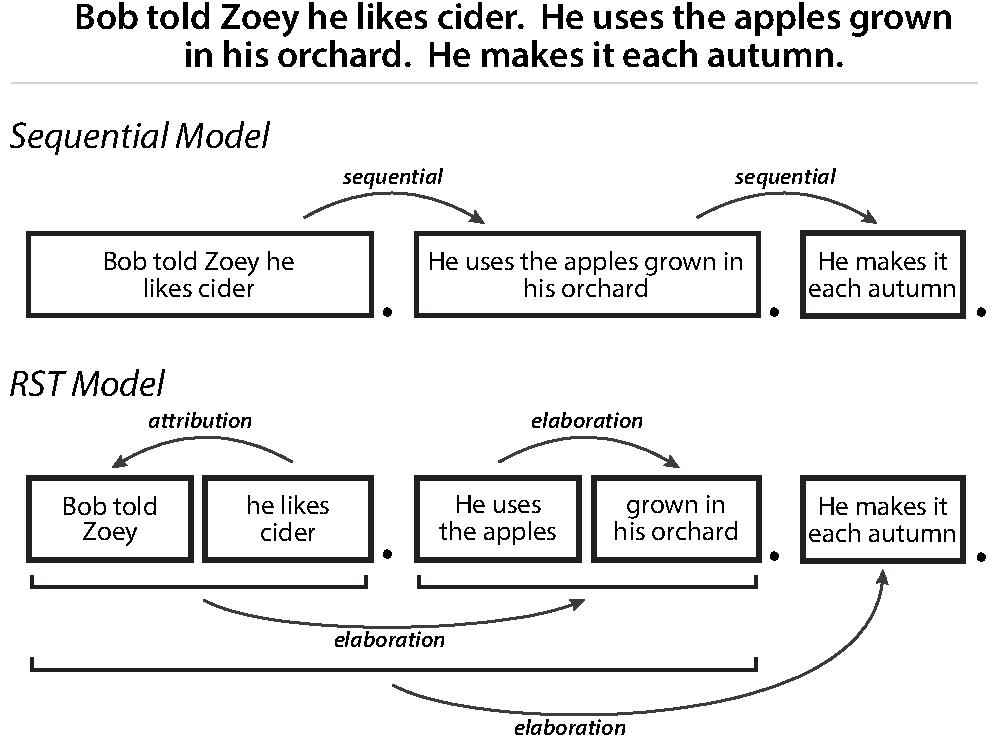
\includegraphics[width=75mm]{mainmatter/naacl2015-alignment/rst2a.pdf}
%space{-2mm}
\caption{{\small An example of the alignments produced by the two discourse models.  The sequential model aligns pairs of consecutive sentences, capturing intersentence associations such as \emph{cider--apples}, and \emph{orchard--autumn}.  The Rhetorical Structure Theory based model generates alignment pairs from participants in all (binary) discourse relations, capturing both intrasentence and intersentence alignments, including 
\emph{apples--orchard, cider--apples}, and \emph{cider--autumn}.}}
\label{fig:examples}
\end{center}
\end{figure}

\section{Approach}
\label{sec-naacl2015:approach}

A written text is not simply a collection of sentences, but rather a flowing narrative where sentences and sentence elements depend on each other for meaning -- a concept known as cohesion~\citep{halliday2014cohesion}.  
Here we examine two methods for generating alignment training data from free text that make use of cohesion: a shallow method that uses only intersentence structures, and a deep method that uses both intrasentence and intersentence structures.
We additionally attempt to separate the contribution of discourse from that of alignment in general by comparing these models against a baseline alignment model which aligns sentences at random.

The first model, the sequential discourse model (SEQ), considers that each sentence continues the narrative  of the previous one, and creates artificial question-answer pairs from all pairs of consecutive sentences.
% ms: no space
%This is similar to a right-attachment baseline in dependency parsing, 
%but operating at sentence granularity rather than word.
Thus, this model takes advantage of intersentence cohesion by aligning the content words\footnote{In pilot experiments, we found that aligning only nouns, verbs, adjectives, and adverbs yielded higher performance.} in each sentence with the content words in the following sentence.  For example, in the passage in Figure \ref{fig:examples}, this model would associate \emph{cider} in the first sentence with \emph{apples} and \emph{orchard} in the second sentence.

The second model uses Rhetorical Structure Theory (RST) to capture discourse cohesion both within and across sentence boundaries.  
We extracted RST discourse structures using an in-house parser~\citep{Surdeanu:15}, which follows the architecture introduced by \citet{hernault10} and \citet{feng12}.
The parser first segments text into elementary discourse units, which may be at sub-sentence granularity, then recursively connects neighboring units with binary discourse relations, such as \emph{Elaboration} or \emph{Contrast}.\footnote{The RST parser performs better on relations which occur more frequently.  We use only relations that occurred at least 1\% of the time.  This amounted to six relations: \emph{elaboration}, \emph{attribution}, \emph{background}, \emph{contrast}, \emph{same-unit}, and \emph{joint}. Using all relations slightly improves performance by 0.3\% P@1.} Our parser differs from previous work with respect to feature generation in that we implement all features that rely on syntax using solely dependency syntax. For example, a crucial feature used by the parser is the dominance relations of \citet{soricut2003}, which capture syntactic dominance between discourse units located in the same sentence. While originally these dominance relations were implemented using constituent syntax, we provide an equivalent implementation that relies on dependency syntax. The main advantage to this approach is speed: the resulting parser performs at least an order of magnitude faster than the parser of \citet{feng12}. 

Importantly, we generate artificial alignment pairs from this imposed structure by aligning the governing text (nucleus) with its dependent text (satellite).\footnote{Pilot experiments showed that this direction of alignment performed better than aligning from satellite to nucleus.} 
 Turning again to the example in Figure \ref{fig:examples}, this RST-based model captures additional alignments that are both intrasentence, e.g., \emph{apples--orchard}, and intersentence, e.g., {\em cider--autumn}. 
% intersentence associations of the sequential baseline, in addition it finds an intrasentence association between \emph{apples} and \emph{orchard}. 

%\todo{The random alignment baseline (RND) was created in a similar fashion to the SEQ model, except that the sentences were randomly shuffled first.  In the open domain this shuffling took place within a document, and in the biology domain it was done across the entire of the textbook.}



%----------------------TABLE FORMAT FROM TACL 2015--------
\begin{table*}[t]{}
        \centering
        \begin{tabular}{p{1cm}p{10cm}}
		\hline        
        \multicolumn{2}{l}{\bf Alignment Models} \\
        \hline
        \multicolumn{2}{l}{Global Alignment Probability:} \\
		  &  p(Q$|$A) according to IBM Model 1 \citep{Brown:93} \\ 
		\\        
        \multicolumn{2}{l}{Jenson-Shannon Distance (JSD) Features:} \\         
         {  } & {Pairwise JSDs were found between the probability distribution of each content word in the question and those in the answer.  The \textbf{mean, minimum, and maximum JSD values} were used as features. Additionally, composite vectors were formed which represented the entire question and the entire answer and the \textbf{overall JSD} between these two vectors was also included as a feature. See \citet{fried2015higher} for additional details.} \\
		\\        
        \hline
		 \multicolumn{2}{l}{\bf Embedding Model} \\
		 \hline
		 \multicolumn{2}{l}{Cosine Similarity Features:} \\        
         {  } & {Similar to \citet{jansen14}, we include as features the {\bf maximum and average pairwise cosine similarity} between question and answer words, as well as the {\bf overall similarity} between the composite question and answer vectors.} \\
        \end{tabular}
        \caption{Feature descriptions for alignment models and the embedding baseline.}
        \label{tab:Features}
	
\end{table*}

%\begin{table*}[h]{}
%
%%\begin{scriptsize}
%
%        \centering
%        %\resizebox{7.9cm}{!}{
%        {
%        %\begin{tabular}{p{1cm}|p{3cm}|l}
%        \begin{tabular}{p{0.3cm}|p{5cm}|p{8cm}}
%        \hspace*{-7pt}  & Feature Group & Feature Descriptions \\
%        \toprule
%        \multirow{10}{*}
%        {\rotatebox[origin=c]{90}{~~~~~~~~~Alignment Models}}
%        & { Global Alignment Probability } & p(Q$|$A) according to IBM Model 1 \cite{Brown:93}\\ 
%        & {} & {}\\
%        & { Jenson-Shannon Distance (JSD) } & {Pairwise JSDs were found between the probability distribution of each content word in the question and those in the answer.  The \textbf{mean, minimum, and maximum JSD values} were used as features. Additionally, composite vectors were formed which represented the entire question and the entire answer and the \textbf{overall JSD} between these two vectors was also included as a feature. See Fried et. al \citeyear{fried2015higher} for additional details.} \\
%        \midrule
%        \multirow{10}{*}
%        {\rotatebox[origin=c]{90}{~~~~~~~~~~~~~~~~~~~~~~~~~~~~~~~~~~RNNLM}}
%        & { Cosine Similarity } & {Similar to Jansen et al.~\citeyear{jansen14}, we include as features the {\bf maximum and average pairwise cosine similarity} between question and answer words, as well as the {\bf overall similarity} between the composite question and answer vectors.} \\
%        \bottomrule
%        \end{tabular}
%        }
%        %}
%
%%\end{scriptsize}
%
%        %\caption{$10$ most important features of each sieve.}
%        \caption{Feature descriptions for alignment models and RNNLM baseline.}
%        \label{tab:Features}
%	\vspace{-6mm}
%
%\end{table*}

%------------------END COPIED TABLE----------------
%space{-1mm}
\section{Models and Features}
\label{sec-naacl2015:models}

We evaluate the contribution of these alignment models using a standard reranking architecture~\citep{jansen14}.
The initial ranking of candidate answers is done using a shallow information retrieval (IR) component.\footnote{We use the same cosine similarity between question and answer lemmas as \citet{jansen14}, weighted using {\em tf.idf}.  Please see \citet{jansen14} for detailed architecture.}  
Then, these answers are reranked using a more expressive model that incorporates alignment features alongside the IR score.  As a learning framework we use \svmr , a Support Vector Machine tailored for ranking.\footnote{ \url{http://www.cs.cornell.edu/people/tj/svm_light/svm_rank.html}}
We compare this alignment-based reranking model against one that uses a state-of-the-art recurrent neural network language model \citep{mikolov10,mikolov13}, which has been successfully applied to QA previously~\citep[e.g.,][]{yih13}.


{\flushleft {\bf Alignment Model:}}  The alignment matrices were generated with IBM Model 1 \citep{Brown:93} using GIZA++~\citep{och03}, and the corresponding models were implemented as per \citet{Surdeanu:11} with a global alignment probability, i.e., the conditional probability of observing a question given an answer.
% ms: the global prob. operates for the whole Q and A!
%question word given an answer word.
\footnote{Within \citet{Surdeanu:11} framework, we lightly tuned the smoothing parameter, $\lambda$, to 0.4 and we redistributed the probability mass for each word such that the probability of a word translating to itself was 0.5.}  
We extend this alignment model with features from \citet{fried2015higher} that treat each (source) word's probability distribution (over destination words) in the alignment matrix as a distributed semantic representation, and make use of the Jensen-Shannon distance (JSD)\footnote{Jensen-Shannon distance is based on Kullback-Liebler divergence but is a distance metric (finite and symmetric).} between these conditional distributions.  A summary of all these features is shown in Table \ref{tab:Features}.% to derive features representing the {\bf minimum, maximum, and average JSDs} between question and answer words, as well as the {\bf overall JSD} between the composite question and answer distributions. 
%Using the Jensen-Shannon distance (JSD) between conditional distributions, content words in each question were compared with the content words in its answers.  Features were made from the maximum, minimum, and average JSDs.  Composite distributions were also created for the entire question and for each entire candidate answer, and the JSD between these composite distributions was used as a feature. 


{\flushleft {\bf Embed:}} We learned word embeddings using the \texttt{word2vec} recurrent neural network language model of \citet{mikolov13}, and include the cosine similarity-based features described in Table \ref{tab:Features}. %Similar to Jansen et al.~\citeyear{jansen14}, we include as features the {\bf maximum and average pairwise cosine similarity} between question and answer words, as well as the {\bf overall similarity} between the composite question and answer vectors. 

%{\flushleft {\bf Hyperparameters}}We used the following very lightly tuned hyperparameters: for \svmr, we used c = 0.1 and for IBM model 1, lambda = 0.4 and self-association of 0.5. \todo{re-write this!! or spread to appropriate places} 

\input{mainmatter/naacl2015-alignment/naacl2015_experiments}
%
%space{-1mm}
\section{Discussion}
\label{sec-naacl2015:discussion}
%space{-2mm}

%
% Alignment performance by part-of-speech association (noun/noun, verb/verb, noun/verb, etc)
%
\begin{comment}
\begin{table}[t!]
\begin{center}
%\begin{scriptsize}
\begin{footnotesize}
\begin{tabular}{llc}
\multicolumn{1}{l}{ } & \multicolumn{1}{l}{ } & \multicolumn{1}{l}{P@1} \\
\multicolumn{1}{l}{ Model/Features } & \multicolumn{1}{l}{P@1} & \multicolumn{1}{l}{Impr.} \\
\cline{2-3}

\hline
\multicolumn{3}{l}{\textit{Yahoo! Answers}} \\ % 185q (sent) ret=1p c=0.1 
\hline
CR Baseline 							& 19.00 					&	  				\\
Full model  							& 29.00 					& +XX\% 			\\
Verb  $\rightarrow$ Verb 				& {\bf XX.XX\ssa}			& {\bf +XX\%}		\\
Verb  $\rightarrow$ Noun 				& {\bf XX.XX\ssa}			& {\bf +XX\%}		\\
Noun  $\rightarrow$ Noun 				& {\bf XX.XX\ssa}			& {\bf +XX\%}		\\

\end{tabular}
%\end{scriptsize}
\end{footnotesize}
%\vspace{-2mm}
\caption{{\footnotesize  Performance of an alignment model trained with only verb$\rightarrow$verb, verb$\rightarrow$noun, or noun$\rightarrow$noun associations on the Y!A corpus.  Performance suggests the effect is primarily driven by XX$\rightarrow$XX associations. 
}}
\label{tab:associationtype}
%\vspace{-4mm}
\end{center}
\end{table}
\end{comment}

The utility of the proposed approach is clear -- by imposing structure over free text,  monolingual alignment can used (with extremely sparse data) to achieve large performance gains in non-factoid QA.  When discourse parsing is possible for the free text in the domain in question, intersentence and intrasentence alignments can be combined to reach maximal performance.  Otherwise, just a straightforward aligning of adjacent sentences can attain a close approximation of those results.  Both of these models far outperform an RNNLM when trained on limited amounts of data.  

In fact, it is notable how quickly we see performance increases from the alignment models in YA.  In both domains, results are increased due to word self-associations (when the same word appears in both the question and the answer), but with YA there also is a slight correlation between answer length and correctness.  The magnitude of the performance increase due to these factors is essentially shown in the results for the smallest sample size, as one document doesn't contain enough data to provide a real alignment contribution.  Taking this into account, the scores still increase quite rapidly for YA.  It could be the case that associations between high frequency verbs drive much of this performance.  If so, then perhaps for the more technical Bio domain, more world-knowledge (encoded in nouns and other parts of speech) is needed,  explaining why we don't see the same immediate performance gain.  To test this, matrices could be made with only verbs, only nouns, or other combinations to determine if one type of association is driving much of the performance and how the domains compare in this respect. 

After a rapid increase, the performance in YA quickly levels off relative to the amount of input for training.~\footnote{Only a fraction of 1 file is used to achieve the maximal performance for the alignment models.  In pilot experiments, including as many as 20 files did not improve performance. }  This may be a result of a decrease in the signal to noise ratio.  Unlike YA, gigaword is within the news domain.  As more and mode documents are added to training, perhaps the model becomes too far biased towards news to continue to increase performance.  If more sophisticated techniques are implemented, such as topic filtering, potentially the performance in this domain could be even higher.  We don't see the same plateau effect with Bio that we do with YA.  Likely this is due to the fact that the in-domain texbook for Bio was much smaller than gigaword.  With more in-domain data we would expect the results for all models to increase, and perhaps the performance curves would resemble those from YA.

\todo{strong close}





%
%space{-1mm}
\section{Discussion}
\label{sec-naacl2015:discussion}
%space{-2mm}

%
% Alignment performance by part-of-speech association (noun/noun, verb/verb, noun/verb, etc)
%
\begin{comment}
\begin{table}[t!]
\begin{center}
%\begin{scriptsize}
\begin{footnotesize}
\begin{tabular}{llc}
\multicolumn{1}{l}{ } & \multicolumn{1}{l}{ } & \multicolumn{1}{l}{P@1} \\
\multicolumn{1}{l}{ Model/Features } & \multicolumn{1}{l}{P@1} & \multicolumn{1}{l}{Impr.} \\
\cline{2-3}

\hline
\multicolumn{3}{l}{\textit{Yahoo! Answers}} \\ % 185q (sent) ret=1p c=0.1 
\hline
CR Baseline 							& 19.00 					&	  				\\
Full model  							& 29.00 					& +XX\% 			\\
Verb  $\rightarrow$ Verb 				& {\bf XX.XX\ssa}			& {\bf +XX\%}		\\
Verb  $\rightarrow$ Noun 				& {\bf XX.XX\ssa}			& {\bf +XX\%}		\\
Noun  $\rightarrow$ Noun 				& {\bf XX.XX\ssa}			& {\bf +XX\%}		\\

\end{tabular}
%\end{scriptsize}
\end{footnotesize}
%\vspace{-2mm}
\caption{{\footnotesize  Performance of an alignment model trained with only verb$\rightarrow$verb, verb$\rightarrow$noun, or noun$\rightarrow$noun associations on the Y!A corpus.  Performance suggests the effect is primarily driven by XX$\rightarrow$XX associations. 
}}
\label{tab:associationtype}
%\vspace{-4mm}
\end{center}
\end{table}
\end{comment}

The utility of the proposed approach is clear -- by imposing structure over free text,  monolingual alignment can used (with extremely sparse data) to achieve large performance gains in non-factoid QA.  When discourse parsing is possible for the free text in the domain in question, intersentence and intrasentence alignments can be combined to reach maximal performance.  Otherwise, just a straightforward aligning of adjacent sentences can attain a close approximation of those results.  Both of these models far outperform an RNNLM when trained on limited amounts of data.  

In fact, it is notable how quickly we see performance increases from the alignment models in YA.  In both domains, results are increased due to word self-associations (when the same word appears in both the question and the answer), but with YA there also is a slight correlation between answer length and correctness.  The magnitude of the performance increase due to these factors is essentially shown in the results for the smallest sample size, as one document doesn't contain enough data to provide a real alignment contribution.  Taking this into account, the scores still increase quite rapidly for YA.  It could be the case that associations between high frequency verbs drive much of this performance.  If so, then perhaps for the more technical Bio domain, more world-knowledge (encoded in nouns and other parts of speech) is needed,  explaining why we don't see the same immediate performance gain.  To test this, matrices could be made with only verbs, only nouns, or other combinations to determine if one type of association is driving much of the performance and how the domains compare in this respect. 

After a rapid increase, the performance in YA quickly levels off relative to the amount of input for training.~\footnote{Only a fraction of 1 file is used to achieve the maximal performance for the alignment models.  In pilot experiments, including as many as 20 files did not improve performance. }  This may be a result of a decrease in the signal to noise ratio.  Unlike YA, gigaword is within the news domain.  As more and mode documents are added to training, perhaps the model becomes too far biased towards news to continue to increase performance.  If more sophisticated techniques are implemented, such as topic filtering, potentially the performance in this domain could be even higher.  We don't see the same plateau effect with Bio that we do with YA.  Likely this is due to the fact that the in-domain texbook for Bio was much smaller than gigaword.  With more in-domain data we would expect the results for all models to increase, and perhaps the performance curves would resemble those from YA.

\todo{strong close}






%space{-2mm}
%\begin{small}
%\section*{Acknowledgments}
%space{-2mm}
%We thank the Allen Institute for AI for funding this work.
%\end{small}

%\bibliographystyle{acl}
%\bibliography{citations} % add your references to citations, then run bibtex

% If you use BibTeX with a bib file named eacl2014.bib, 
% you should add the following two lines:
%\bibliographystyle{acl}
%\bibliography{acl2014}
%\bibliography{refs}
%\bibliography{citations}


\input{mainmatter/emnlp2016-causal/emnlp2016_main}
\input{mainmatter/tacl2015-tig/cl2017_main}
% Our packages
%\usepackage{float}
%\usepackage[font=small]{caption}
%\usepackage{color}
%\usepackage{graphicx}
%\usepackage{booktabs}
%\usepackage{subcaption}
%\usepackage{hyperref}
%\usepackage[utf8]{inputenc}
%\usepackage{tabularx}
%\usepackage{tablefootnote}
%\usepackage{amsmath}
%\usepackage{amssymb}
%\usepackage{placeins}
%\usepackage{scrextend}

%\title{Tell Me Why: Using Question Answering as Distant Supervision for Answer Justification}


%\begin{abstract}
%
%For many applications of question answering (QA), being able to explain why a given model chose an answer is critical.  However, the lack of labeled data for  answer justifications makes learning this difficult and expensive.  Here we propose an approach that uses answer ranking as distant supervision for learning how to select informative justifications. 
%We propose a neural network architecture for QA that reranks answer justifications as an intermediate (and human-interpretable) step in answer selection. Our approach is informed by a set of features designed to combine both learned representations and explicit features to capture the connection between questions, answers, and answer justifications.
% We show that with this end-to-end approach we are able to significantly improve upon a strong IR baseline in both justification ranking (+9\% rated highly relevant) and answer selection (+6\% P@1).  %We also provide an error analysis that demonstrates that we can use the justifications returned to better understand what our model has learned.
%\end{abstract}

\chapter{EMNLP2017 - QAJ\label{chapter:emnlp2017}}

%\section{Introduction}
\label{sec-emnlp2017:intro}

Developing interpretable machine learning (ML) models, that is, models where a human user can \emph{understand} what the model is learning, is considered by many to be crucial for ensuring usability and accelerating progress \cite{craven1996extracting,Kim2015MindTG, letham2015interpretable, Ribeiro2016WhySI}.  
% bs: removed for space, we talk more about this in related work
%As such, it has received much attention in recent years, especially as deep learning and complex architectures have seen dramatic gains in many tasks.
For many applications of question answering (QA), i.e., finding short answers to natural language questions, simply providing an answer is not sufficient. A complete approach must be interpretable, i.e., able to {\em explain} why an answer is correct. 
For example, in the medical domain, a QA approach that answers treatment questions would not be trusted if the treatment recommendation is not explained in terms that can be understood by the human user. 


One approach to interpreting complex models is to make use of human-interpretable information % metric % ms: not a metric...
 generated by the model to gain insight into what the model is learning.  This can be an intermediate representation used by the model, as with the model-generated text spans of \citet{Lei2016RationalizingNP}, that serve as input to another classification network.  
By learning these intermediate representations end-to-end with a downstream task, they are optimized to correlate with what the model learns is discriminatory for the task, and they can be evaluated against what a human would consider to be important.
\todo{need to define what a downstream task means to use this term}, they are optimized to correlate with what the model learns is discriminatory for the task, and they can be evaluated against what a human would consider to be important.
Here we apply this general framework for model interpretability to QA.


\begin{table}[t]
\begin{center}
\begin{footnotesize}
\begin{tabularx}{\linewidth}{p{0.13cm}p{6.8cm}}
\multicolumn{2}{p{8cm}}{\textbf{Question:} Which of these is a response to an internal stimulus?} \\
 (A) & A sunflower turns to face the rising sun. \\
 (B) & A cucumber tendril wraps around a wire. \\
 (C) &  A pine tree knocked sideways in a landslide grows upward in a bend. \\
 (\textbf{D}) &\textbf{Guard cells of a tomato plant leaf close when there is little water in the roots .} \\
\\
\multicolumn{2}{p{7.2cm}}{\textbf{Justification:} 
Plants rely on hormones to send signals within the plant in order to respond to internal stimuli such as a lack of water or nutrients. } \\

\end{tabularx}
\end{footnotesize}
\caption{{  Example of an 8th grade science question with a justification for the correct answer.  Note the lack of direct lexical overlap present between the justification and the correct answer, demonstrating the difficulty of the task of finding justifications using traditional distant supervision methods. }}
%space{-6mm} 
\label{tab:question_example}
\end{center}
\end{table}

In this work, we focus on answering multiple-choice science exam questions (Clark \citeyear{clark:2015}; see example in Table~\ref{tab:question_example}). 
This domain is challenging as: (a) approximately 70\% of science exam question shave been shown to require complex forms of inference to solve \cite{clark:2013,jansen-EtAl:2016:COLING}, and (b) there are few structured knowledge bases to support this inference.  
Within this domain, we propose an approach that learns to both select and explain answers, when the only supervision available is for which answer is correct (but not how to explain it).
Intuitively, our approach chooses the justifications that provide the most help towards ranking the correct answers higher than incorrect ones.
More formally, our neural network approach alternates between using the current model with max-pooling to choose the highest scoring justifications for correct answers, and optimizing the answer ranking model given these justifications. 
Crucially, these reranked texts serve as our human-readable answer justifications, and by examining them, we gain insight into what the model learned was useful for the QA task.   


The specific contributions of this work are:
\begin{enumerate}
\item We propose an end-to-end neural method for learning to answer questions and select a high-quality justification for those answers. 
Our approach re-ranks free-text answer justifications without the need for structured knowledge bases. 
With supervision only for the correct answers, we learn this re-ranking through a form of distant supervision -- i.e., the answer ranking supervises the justification re-ranking. 

\item We investigate two distinct categories of features in this ``little data'' domain: explicit features, and learned representations. We show that, with limited training, explicit features perform far better despite their simplicity. 

\item We demonstrate a large (+9\%) improvement in generating high-quality justifications over a strong information retrieval (IR) baseline, while maintaining near state-of-the-art performance on the multiple-choice science-exam QA task, demonstrating the success of the end-to-end strategy.
\end{enumerate}

%\input{mainmatter/emnlp2017-qaj/emnlp2017_related}
\section{Balancing interpretability with robustness: A neural approach to reranking justifications}
\label{sec-emnlp2017:intro}

In many ways, deep learning has become the canonical example of the "black box" of machine learning and many of the approaches to explaining it can be loosely categorized into two types: approaches that try to interpret the parameters themselves (e.g., with visualizations and heat maps \citep{Zeiler2014VisualizingAU,nips15_hermann, Li2016VisualizingAU}, and approaches that generate a human-interpretable metric that is ideally correlated with what is being learned inside the model (e.g., \citet{Lei2016RationalizingNP}). Our approach falls into the latter type -- 
we use our model's reranking of human-readable justifications to give us insight into what the model considers informative for answering questions.  This allows us to see where we do well (Section \ref{sec:justification_results}), and where we can improve (Section  \ref{sec:erroranalysis}).

Deep learning has been successfully applied to many recent QA approaches and related tasks \citep[][inter alia]{Bordes2015LargescaleSQ,nips15_hermann, He2016CharacterLevelQA, dong2015question, Tan2016ImprovedRL}.
However, large quantities of data are needed to train the millions of parameters often contained in these models.  
Recently, simpler model architectures have been proposed that greatly reduce the number of parameters while maintaining high performance \cite[e.g.,][]{Iyyer2015,chen2016thorough,Parikh2016ADA}.  
%For example, \citet{Iyyer2015}'s show that with their Deep Averaged Network, which replaces complex recurrent neural networks with an average of embeddings and a few, albeit large, dense layers, they improved performance on both a sentiment analysis and a QA task.  For natural language inference, \citet{Parikh2016ADA} used a simpler neural alignment  approach with an attention mechanisms to greatly reduce the size of their model while reaching then state-of-the-art performance.  
We take inspiration from this trend and propose a simple neural architecture for our task to offset the limited available training data. 

Another way to mitigate sparse training data is to include higher-level explicit features.  Like \citet{sachan2016science}, we make use of explicit features alongside features from distributed representations to capture connections between questions, answers, and supporting text.  However, we use a simpler set of features and while they use structured and semi-structured knowledge bases, we use only free-text.  %Additionally, though we also learn to select support from our knowledge base (in some ways similar to \citeauthor{sachan2016science}'s latent answer-entailing structure), since we are explicitly trying to perform \emph{explainable} question answering, here we evaluate the justifications learned by our approach and show that they are significantly better than a  strong IR baseline (Section \ref{sec:justification_results}).   

Our approach to learning justification reranking end-to-end with answer selection is similar to the \citet{jansen2017framing} latent reranking perceptron,  which also operates over free text.  However, our approach does not require decomposing the text into an intermediate representation, allowing our technique to more easily extend to larger textual knowledge bases.  

 


%\todo{Discriminative information retrieval for question answering sentence selection(Chen and Van-Durme): Presented a method that selects sentences which contain potential answers for questions from a very large corpus (10\^7 sentences, requiring several thousand questions for training). Their results are dramatically better than Lucene across two datasets and several evaluation measures.}
%(Yih et al.,2013; Wang and Manning, 2010; Heilman and Smith, 2010; Yao et al., 2013a) and recently using neural networks (Yu et al., 2014; Severyn and Moschitti,2015; Wang and Nyberg, 2015; Yin et al.,2016)


\begin{figure}[t]
\begin{center}
\includegraphics[width=0.5\textwidth]{mainmatter/emnlp2017-qaj/arch_overall.png}
\caption{ Architecture of our question answering approach.  
Given a question, candidate answer, and a free-text knowledge base as inputs, we generate a pool of candidate justifications, from which we extract feature vectors.  We use a neural network to score each and then use max-pooling to select the current best justification. This serves as the score for the candidate answer itself.  The red border indicates the components that are trained online. }
\label{fig:arch_overall}
%space{-5mm}
\end{center}
\end{figure}

\section{Approach}
\label{sec-emnlp2017:approach}
One of the primary difficulties with the explainable QA task addressed here is that, while we have supervision for the correct answer, we do not have annotated answer justifications.  
Here we tackle this challenge by using the QA task performance as supervision for the justification reranking, allowing us to 
%extending a neural QA model to jointly learn both how to 
%jointly 
learn to choose both the correct answer and a compelling, human-readable justification for that answer.

Additionally, similar to the strategy Chen and Manning~\citeyear{chen2014fast} applied to parsing, we combine representation-based features with explicit features that capture additional information that is difficult to model through embeddings, especially with limited training data.
%second contribution is that, similar to the strategy Chen and Manning~\citeyear{chen2014fast} applied to parsing, we combine representation-based features with explicit features that capture additional information that is difficult to model through embeddings.



% ms: avoid "system" too engineering-y
The architecture of our approach is summarized in Figure \ref{fig:arch_overall}.  
Given a question and a candidate answer, we first query an textual knowledge base (KB) to retrieve a pool of potential justifications for that answer candidate.  
For each justification, we extract a set of features designed to model the relations between questions, answers, and answer justifications based on word embeddings, lexical overlap with the question and answer candidate, discourse, and information retrieval (IR) (Section \ref{sec-emnlp2017:features}).
These features are passed into a simple neural network to generate a score for each justification, given the current state of the model.  A final max-pooling layer selects the top-scoring justification for the candidate answer and this max score is used also as the score for the answer candidate.  
The system is trained using correct-incorrect answer pairs with a pairwise margin ranking loss objective function to enforce that the correct answer be ranked higher than any of the incorrect answers. 

%The key here is that we use the current state of the model to select the best justification for a given answer candidate from a pool of many candidate justifications.  To do this, we modify the training procedure such that at the start of each epoch \todo{minibatch instead of epoch?}, we first compute a forward pass with each candidate justification to find the top-scoring justification for each candidate answer.
%For a given question, answer candidate, and justification, we combine features based on word embeddings, lexical overlap, discourse, and information retrieval (IR) together in a simple neural architecture to generate a score for the answer candidate.    We then use this selected justification to calculate our gradients for updating the model parameters.  

With this end-to-end approach, the model learns to select justifications that allow it to correctly answer questions.  We hypothesize that this approach enables the model to indirectly learn to choose justifications that provide good explanations as to why the answer is correct. We empirically test this hypothesis in Section \ref{sec-emnlp2017:results}, where we show that indeed the model learns to correctly answer questions, as well as to select high-quality justifications for those answers. 
% ms: misleading; it reads as if answer selection is better than IR
% better than a strong IR baseline. 


\begin{figure}[t]
\begin{center}
\includegraphics[width=0.8\textwidth]{mainmatter/emnlp2017-qaj/ArchDiagram.png}
\caption{ Detailed architecture of the model's scoring component.  
The question, candidate answer, and justification %\edit{(previously obtained through max-pooling)}
% bs: no - the max pooling happens at the end, after the scoring. 
 are encoded (by summing their word embeddings) to create vector representations of each. These representations are combined in several ways to create a set of representation-based similarity features that are concatenated to additional explicit features capturing lexical overlap, discourse and IR information and fed into a feed-forward neural network.  The output layer of the network is a single node that represents the score of the justification candidate.}  %\todo{Take out? As described in Section \ref{sec-emnlp2017:approach}, we then use max-pooling over these justification scores to assign a score to the answer candidate itself.} }
 %bs: sure -- it's shown in the arch right next door :)
\label{fig:arch}
%space{-5mm}
\end{center}
\end{figure}


\section{Model and Features}
\label{sec-emnlp2017:pipeline}
%\bs{we're low on space and I'm not sure we really need all the features in table 2... in fact, do we need the table at all? \\similarity features are described in prose, as are discourse features (and example is in sep figure), and IR++ features.  Should we remove the table and move the description of LO features to prose? we could recapture half a column...}.  
% removed table per mihai email
Our approach consists of three main components: (a) the retrieval of a pool of candidate answer justifications (Section \ref{sec-emnlp2017:justretrieval}); (b) the extraction of features for each (Section \ref{sec-emnlp2017:features}); and (c) the scoring of the answer candidate itself based on this pool of justifications (Section \ref{sec-emnlp2017:nn_model}).  The architecture of this latter scoring component is shown in Figure \ref{fig:arch}. 


\begin{table}[h!]
\begin{center}
\begin{footnotesize}
\begin{tabular}{p{0.5cm}p{12cm}}
%\hline
%Feature  & Description \\ 
\hline
\multicolumn{2}{l}{Representation-Based Features (Emb)} \\
\hline
\multicolumn{2}{l}{$sim(Q,A)$, $sim(Q,J)$, and $sim(Q,J)$} \\
  & The pairwise cosine similarities between the question, answer, and justification representations. \\
\multicolumn{2}{l}{$sim(Q, uniqueJ)$ and $sim(A, uniqueJ)$} \\
& The cosine similarities between each of the question and answer representations and the representation for the terms in the justification which don't overlap with either. \\
\multicolumn{2}{l}{$dist(Q + J, A)$} \\
 & The euclidean distance between the sum of the question and justification representations and that of the answer (see Section \ref{sec-emnlp2017:features} for motivation and details).\\
\hline
\multicolumn{2}{l}{Lexical Overlap Features (LO)} \\
\hline
\multicolumn{2}{l}{\emph{qCoverage}, \emph{aCoverage}, and \emph{qaCoverage}} \\
 & The proportion of question words, of answer words, and of the combined set of question and answer words that also appear in the justification. \\
% & The proportion of answer words that also appear in the justification. \\
% & The proportion of combined question and answer words that also appear in the justification. \\ 
\multicolumn{2}{l}{\emph{jNovelty}} \\
 & The proportion of justification words that do not appear in either the question or the answer. \\
\multicolumn{2}{l}{\emph{numWords}} \\
 & Length of the justification in words.\tablefootnote{We normalized this value by the maximum justification length.} \\

\hline
\multicolumn{2}{l}{Semi-Lexicalized Discourse Features (lexDisc)} \\
\hline
\multicolumn{2}{l}{\emph{lexDisc$_0$, ..., lexDisc$_n$}} \\
 & A set of indicator-like features that capture the presence of semi-lexicalized discourse relations (see Section \ref{sec-emnlp2017:features} for details and example). \\
 \hline
\multicolumn{2}{l}{IR-Based Features (IR$^{++}$)} \\
\hline
\multicolumn{2}{l}{\emph{IR$_{max}$, IR$_{sum}$}} \\
 & The reciprocal rank of the answer candidate based on (a) the highest scoring IR-retrieved document and (b) the weighted sum of all the IR-retrieved documents, using the basic IR query (see \ref{sec-emnlp2017:features} for details).\\
\multicolumn{2}{l}{\emph{IR$_{max}^{boosted}$, IR$_{sum}^{boosted}$}} \\
 & The reciprocal rank of the answer candidate based on (a) the highest scoring IR-retrieved document and (b) the weighted sum of all the IR-retrieved documents, using the boosted IR query (see \ref{sec-emnlp2017:features} for details). \\

\end{tabular}
\end{footnotesize}
\caption{{ Summary of the features calculated for each candidate justification.  
 }} 
\label{tab:feature_examples}
\end{center}
\end{table}

\subsection{Candidate Justification Retrieval}
\label{sec-emnlp2017:justretrieval}
The first step in our process is to use standard information retrieval (IR) methods to retrieve a set of candidate justifications for each candidate answer to a given question.  To do this, we build a bag-of-words query using the content lemmas for the question and answer candidate, boosting the answer lemmas to have four times more weight\footnote{We empirically found this answer term boosting to ensure retrieval of documents which were relevant to the particular answer candidate.}.  We used Lucene\footnote{\url{https://lucene.apache.org}} with a \emph{tf-idf} based scoring function to return the top-scoring documents from the knowledge base.  Each of these indexed documents consists of a single sentence from our corpora, and serves as one potential justification.  
%\todo{Say here that each Lucene document indexes one potential justification, i.e., one sentence from X, or one paragraph from Y?}

\subsection{Feature Extraction}
\label{sec-emnlp2017:features}
For each retrieved candidate justification, we extract a set of features based on (a) distributed representations (i.e., word embeddings) of the question, candidate answer, and justification terms; (b) strict lexical overlap; (c) discourse relations present in the justification; and (d) the IR scores for the justification.  Each of these features is described in detail below, and a summary is provided in Table \ref{tab:feature_examples}.

{ \flushleft{\bf Representation-based features (Emb):}} To model the similarity between the text of each question ($Q$), candidate answer ($A$), and candidate justification ($J$), i.e. the answer passage from the IR model, we include a set of features that utilize distributed representations of the words found in each.
%\todo{Needs to explain where the justification vector comes from (e.g. answer passage from IR model)} 
%bs: I disagree -- I think it's pretty clear from 4.1 above.  I added "text" above to make it clearer.  sorry - but we have no space!!!
First we encode each 
%we make a single vector representation for each of the question ($Q$), answer candidate ($A$), and justification ($J$) 
by summing the word embedding vectors for each of their words.\footnote{While this bag-of-words approach is not ideal in many ways, it performed equivalently to far more complicated approaches such as LSTMs and GRUs, also noted by \citep{Iyyer2015}, likely due to the limited training data in this domain.}.  We then compute $sim(Q, A)$, $sim(Q, J)$, and $sim(A, J)$ using cosine similarity.  Using another vector representation of only the \emph{unique} words in the justification, i.e., the words that do not occur in either the question or the candidate answer, we also compute $sim(Q, uniqueJ)$ and $sim(A, uniqueJ)$.  

To create a feature which captures the relationship between the question, answer, \emph{and} justification, we take inspiration from TransE, a popular relation extraction framework \citep{Bordes2013TranslatingEF}.  TransE is based on the premise that if two entities, $e_1$ and $e_2$ are related by a relation $r$, then a mapping into $k$ dimensions, $m(x) \in \mathbb{R}^k$ can be learned such that $m(e_1) + m(r) \approx m(e_2)$.  Here, we modify this intuition for QA by suggesting that given the vectorized representations of the question, answer candidate, and justification above, $Q + J \approx A$, i.e., a question combined with a strong justification will point towards an answer.  Here we model this as an explicit feature, the euclidean distance between $Q + J$ and $A$, and hypothesize that as a consequence the model will learn to select passages that maximize the quality of the justifications.
%Thus, we calculate a feature which is the euclidean distance between $Q + J$ and $A$.  Our intuition is that a question combined with a strong justification will point towards an answer.  Here we model this as an explicit feature, and hypothesize that as a consequence the model will learn to select passages that maximize the quality of the justifications.
This makes a total of six features based on distributed representations. %\todo{This is an important theoretical idea, and should be explicitly stated. e.g. (Our intuition is that a question combined with a strong justification will point towards an answer.  Here we model this as an explicit feature, and hypothesize that as a consequence the model will learn to select passages that maximize the quailty of the justifications.)}  

{\flushleft{\bf Lexical overlap features (LO):}} 
%\todo{This is not a great name, because the next features are also explicit... Maybe, lexical overlap features} 
We additionally characterize each justification in terms of a simple set of explicit features designed to capture the size of the justification, as well as the lexical overlap (and difference) between the justification and the question and answer candidate.  We include these five features: the proportion of question words, of answer words, and of the combined set of question and answer words that also appear in the justification; the proportion of justification words that do not appear in either the question or the answer; and the length of the justification in words.\footnote{We normalized this value by the maximum justification length.} 
%The full set of LO features are shown in Table \ref{tab:feature_examples}.


\begin{figure}[t]
\begin{center}
\includegraphics[width=0.8\textwidth]{mainmatter/emnlp2017-qaj/DiscourseExample.png}
\caption{Example showing the discourse feature extracted from a question, answer, and justification.  Words occurring in the question are shown in blue and words occurring in the answer are shown in green.  The boxes around the justification text indicate the elementary discourse units identified by the discourse parser, and the arrow indicates the found discourse relation (with the assigned relation label given in red). }
\label{fig:discourseexample}
\vspace{-5mm}
\end{center}
\end{figure}

{\flushleft{\bf Semi-Lexicalized Discourse features (lexDisc):}}  These features use the discourse structure of the justification text, which has been shown to be useful for QA~\citep[][see also Chapter \ref{chapter:naacl2015}]{jansen14,sharp-EtAl:2015:NAACL-HLT, sachan2016science}. %, to generate a set of explicit discourse features.  

We use the discourse parser of \citet{Surdeanu:15} to first fragment the text into elementary discourse units (EDUs) and then recursively connects neighboring EDUs together, assigning each a binary discourse relation label such as \emph{Elaboration} or \emph{Contrast}. Each of these discourse relations consists of a head, a relation label, and a modifier. 
%which is based on the architecture of \citet{hernault10} and \citet{feng12}.  This parser first parses each justification into its elementary discourse units (EDUs) and then recursively connects neighboring EDUs together, assigning each a binary discourse relation label such as \emph{Elaboration} or \emph{Contrast}. Each of these discourse relations consists of a head, a relation label, and a modifier.  
%
For each of the 18 possible relation labels (listed in Table \todo{make table in naacl paper chapter}), we create 
a set of semi-lexicalized discourse features that indicate the presence of a given discourse relation as well as whether or not the head and modifier texts contain words from the question and/or the answer.  %This is similar to the discourse-based features of \citet{sachan2016science}, which were the concatenation of the question word (i.e., \emph{why} or \emph{how}) to the relation labels of background sentences.   

Consider, for example, the question \emph{Q: What makes water a good solvent...?  A: strong polarity} shown in Figure \ref{fig:discourseexample}.  The discourse parser identified a causal relation in the justifcation:  [{\em Water is an efficient solvent}]$_{e1}$ [{\em because of this polarity.}]$_{e2}$.  From this discourse relation, we create the semi-lexicalized feature \emph{Q}\_\emph{cause}\_\emph{A}, because there is a {\em Cause} relation between EDUs $e1$ and $e2$, $e1$ overlaps lexically with the question (i.e. \textit{water} and \textit{solvent}}, and $e2$ overlaps lexically with the answer (i.e., \textit{polarity}).
%For example, for the justification [{\em Water is an efficient solvent}]$_{e1}$ [{\em because of this polarity.}]$_{e2}$, we create the semi-lexicalized feature \emph{Q\_cause\_A}, because there is a {\em Cause} relation between EDUs $e1$ and $e2$, $e1$ overlaps with the question ({\em What makes water a good solvent...?}), and $e2$ overlaps with the answer ({\em strong polarity}).
Since there are 18 possible discourse relation labels, and the prefix and suffix can be any of \emph{Q, A, QA} or \emph{None}, this creates a set of 288 indicator features\footnote{In practice these features can be greater than 1.0.  We wanted to maintain the indicator-like quality of the features while still capturing if a given justification contains several of a certain type of discourse feature.  Thus, we use the fourth-root of the count of each of the discourse features present in the justification as the feature value.}, though in practice many combinations are never found.


%
%Consider the example in Figure \ref{fig:discourseexample}, where the justification contains a \emph{Cause} relation whose head contains question words (shown in blue) and whose modifier contains answer words (shown in green).  This corresponds to the semi-lexicalized feature \emph{Q\_cause\_A}.  Since there are 18 possible discourse relation labels, and the prefix and suffix can be any of \emph{Q, A, QA} or \emph{None}, this creates a set of 288 indicator features

{\flushleft{\bf IR-based features (IR$^{++}$):}} 
%\todo{rework in consideration of query details above}
Finally, we also use a set of four IR-based features which are assigned at the level of the answer candidate (i.e., these features are identical for each of the candidate justifications for that answer choice).   
%Given a question and answer candidate, we query the IR system with the content lemmas from both.  
Using the same query method as described in Section \ref{sec-emnlp2017:justretrieval}, for each question and answer candidate we retrieve a set of indexed documents.
Using the \emph{tf-idf} based retrieval scores of these returned documents, 
$s(d_i)$ for $d_i \in D$, we rank the answer candidates using two methods: 
\begin{itemize}
\item by the maximum retrieved document score for each candidate, and  
\item by the weighted sum of all retrieved document scores\footnote{Weighted sum was based on the IR scores used in the winning Kaggle system from user Cardal (\scriptsize{ \url{https://github.com/Cardal/Kaggle_AllenAIscience}})}:

\begin{equation}
\sum_{d_i \in D} \dfrac{1}{i} s(d_i) 
\end{equation}

\end{itemize}
We repeat this process using an unboosted query as well, for a total of four rankings of the answer candidates.  
We then use these rankings to make a set of four reciprocal rank features,  IR$^{++}_0$, ..., IR$^{++}_3$, for each answer candidate (i.e., IR$^{++}_0 = 1.0$ for the top-ranked candidate in the first ranking,  IR$^{++}_0 = 0.5$ for the next candidate, etc.)
%For each answer candidate, we use its position in each of the four rankings above to make a reciprocal rank feature -- these are the IR$^{++}$ features. 
  
%For each of these four IR-based rankings of the answer candidates, We transform these four IR-based rankings into a set of four reciprocal rank features for each answer candidate. 


\subsection{Neural Network}
\label{sec-emnlp2017:nn_model}

As shown in Figure \ref{fig:arch}, the extracted features for each candidate justification are concatenated and passed into a fully-connected feed-forward neural network.  The output layer is a single node representing the justification score.  We then use max-pooling over these scores to select the current best justification for the answer candidate, and use its score as the score for the answer candidate itself.  For training, the correct answer for a given question is paired with each of the incorrect answers, and each are scored as above.  We compute the pair-wise margin ranking loss for each training pair:

\begin{equation}
L = \max(0, m - F(a^{+}) + F(a^{-}))
\end{equation}

where $F(a^+)$ and $F(a^-)$ are the model scores for a correct and incorrect answer candidate and $m$ is the margin, and backpropagate the gradients.
At testing time, we use the trained model to score each answer choice (again using the maximum justification score) and select the highest-scoring.

As we are interested in not only correctly answering questions, but also selecting valid justification for those answers, we keep track of the scores of \emph{all} justifications and use this information to return the top $k$ justifications for each answer choice.  These are evaluated along with the answer selection performance in Section \ref{sec-emnlp2017:results}.

\input{mainmatter/emnlp2017-qaj/emnlp2017_experiments}
\begin{table}[t!]
\begin{center}
\begin{footnotesize}
\begin{tabular}{llll}
\hline
\# & Model & P@1 Val & P@1 Test \\ 
%\hline
%& Baselines & \\
\hline
1	&	Random 			&			25			&  25	\\
2	&	IR Baseline		&			47.2			&	 47	\\
3	&	IR$^{++}$ 		&			50.7$^{**}$			& 36.35	\\
4 & \citet{Iyyer2015}
%\tablefootnote{Our implementation of the architecture described in the paper, using the same embeddings we used with our model and dense layers of equal dimension to our embeddings.} 
& -- & 32.52\\
5 & \citet{khot2017tupleinf} & -- & 46.17 \\
%\hline
%	&	Our Approach & 	&	\\
\hline
6 & Our approach w/o IR	&	50.54$^*$	& 48.66 \\
%7	&	IR$^{++}$ + EF 					&		53.4$^{**\dagger\dagger}$				& 53.4$^{**}$	\\
%8	&	IR$^{++}$ + EF + lexDisc 	&		53.6$^{**\dagger\dagger}$				& 53.42$^{**\dagger}$ 	\\
7	&	Our approach  &	{\bf 54.0}$^{**\dagger\dagger}$		& {\bf 53.3}$^{**\dagger}$ 	\\
\end{tabular}
\end{footnotesize}
%space{-1mm}
\caption{{ Performance on the AI2 Kaggle questions, measured by precision-at-one (P@1).  $^*$s  indicate that the difference between the corresponding model and the IR baseline is statistically significant ($^*$ indicates $p < 0.05$ and $^{**}$ indicates $p < 0.001$) and $^{\dagger}$s  indicate significance compared to IR$^{++}$,
%that the difference between the corresponding model and the IR$^{++}$ baseline is statistically significant. %($^\dagger$ corresponds to $p < 0.05$ and $^{\dagger\dagger}$ corresponds to $p < 0.001$).  
All significance values were determined through a one-tailed bootstrap resampling test with 100,000 iterations. }} 
\label{tab:p@1}
\end{center}
\end{table}

\begin{table}[t!]
\begin{center}
\begin{footnotesize}
\begin{tabular}{ll}
\hline
 Ablated Model & P@1 Val \\ 
\hline
 %LO + lexDisc + Emb	&	50.54$^*$ \\
    %Baseline IR$^{++}$ 							&		50.7$^{**}$	\\
	IR$^{++}$ + LO 					&		53.4$^{**\dagger\dagger}$\\
	IR$^{++}$ + LO + lexDisc 	&		53.6$^{**\dagger\dagger}$ \\
    Full Model (IR$^{++}$ + LO + lexDisc + Emb)  &	{\bf 54.0}$^{**\dagger\dagger}$	\\
\end{tabular}
\end{footnotesize}
%space{-1mm}
\caption{{ Ablation of feature groups results, measured by precision-at-one (P@1) on validation data.  Emb indicates our embedding-based features, LO indicates our lexical overlap features, lexDisc signifies our semi-lexicalized discourse features, and IR$^{++}$ indicates our information retrieval based features.  Significance is indicated as in Table \ref{tab:p@1}.}} 
\label{tab:ablation}
%space{-5mm}
\end{center}
\end{table}

\section{Results}
\label{sec-emnlp2017:results}

Rather than seeking to outperform all other systems at selecting the correct answer to a question, here we aimed to construct a system  that can produce substantially better justifications for why the answer choice is correct to a human user (i.e., that is interpretable), without unduly sacrificing accuracy on the answer selection task (i.e., that maintains robustness).  Accordingly, we evaluate our system both in terms of it's ability to correctly answer questions (Section \ref{sec-emnlp2017:accuracy}), as well as provide high-quality justifications for those answers (\ref{sec-emnlp2017:justification_results}).  Additionally, we perform an error analysis (Section \ref{sec-emnlp2017:erroranalysis}), taking advantage of the insight the reranked justifications provide into what the model is learning.
% \todo{not sure what this sentence means?}.
% bs: is this clearer?

\subsection{QA Performance}
\label{sec-emnlp2017:accuracy}
We evaluated the accuracy of our system as well as the baselines on the held-out 800 set of test questions.  Performance, measured in precision at 1 \citep[P@1;][]{manning08}, is shown in Table \ref{tab:p@1} for both the validation (i.e., cross validation on training) and test partitions.  Because NNs are sensitive to initialization, each experimental result shown is the average performance across five runs, each using different random seeds.   

The best performing baseline on the validation data was a model using only IR$^{++}$ features (line 3), but its performance dropped substantially when evaluated on test due to the failure of several random seed initializations to learn.  For this reason, we assessed significance of our model combinations with respect to both the IR baseline as well as the IR$^{++}$ (indicated by $^*$ and $^{\dagger}$s, respectively). All significance values were determined through a one-tailed bootstrap resampling test with 100,000 iterations (see Section \ref{sec-naacl2015:results}, Footnote \ref{footnote:bootstrap} for implementation).
%For this reason, we assessed significance of our model combinations with respect to both the IR baseline (indicated by $^*$) as well as the IR$^{++}$ system (indicated by $^{\dagger}$s).

Our full model that combines IR$^{++}$, lexical overlap, discourse, and embeddings-based features, has a P@1 of 53.3\% (line 7), an absolute gain of 6.3\% over the strong IR baseline despite using the same background knowledge.  
% + LO + lexDisc + Emb\todo{use the text description to make it easier for the reader, e.g. (that combines IR++ with lexical overlap, ...}, has a P@1 of 53.3, an absolute gain of 6.3\% over the strong IR baseline despite using the same background knowledge.  

%\subsubsection{Comparison to Previous Work}
%\begin{flushleft}
%{\bf Comparison to Previous Work}
%space{-1mm}
%\end{flushleft}
\paragraph{Comparison to Previous Work:}
We compared our performance against another model that achieves state of the art performance on a different set of 8th grade science questions, \textsc{TupleInf}(T+T') \citep{khot2017tupleinf}.  \textsc{TupleInf}(T+T') uses Integer Linear Programming to find support for questions via tuple representations of KB sentences\footnote{Notably, one portion of the tuple KB used was constructed based on a different 8th grade question set than the one we use here.}.
%with structured Open IE \citep{Banko2007OpenIE} tuple representations of both questions and knowledge-base sentences to assess how well a given answer choice is entailed or supported.  
On our test data, \textsc{TupleInf}(T+T') achieves 46.17\% P@1 (line 5). 
%\todo{move back to 1 sigdig?}.  
As this model is independent of an IR component, we compare its performance against our full system without the IR-based features (line 6), whose performance is 48.66\% P@1, an absolute improvement of 2.49\% P@1 (5.4\% relative) despite our unstructured text inputs and the far smaller size of our knowledge base (three orders of magnitude). 

%Notably, their KB used by \citeauthor{khot2017tupleinf} is three orders of magnitude larger than ours.  
%Waterloo -- 280GB, ours is SS+QZ -- 72.5MB

\citet{sachan2016science} also tackle the AI2 Kaggle question set with an approach  that learns alignments between questions and structured and semi-structured KB data.
%They reframe the task as answer entailment and learn alignments between structured and semi-structured KB data and the question-answer hypothesis.  
They use only the training questions (splitting them into training, validation, and testing partitions), supplemented by questions found in online study guides, and report an accuracy of 47.84\%.  By way of a loose comparison (since we are evaluating on different data partitions), our model has approximately 5\% higher performance despite our simpler set of features and unstructured KB.  

We also compare our model to our implementation of the basic Deep-Averaged Network (DAN) Architecture of \citet{Iyyer2015}.  %To ensure a more fair comparison, 
We used the same 50-dimensional embeddings in both models, so with the reduced embedding dimension, we reduced the size of each of the DAN dense layer to 50 as well.  For simplicity, we also did not implement their word-dropout, a feature that they reported as providing a performance boost. Using this implementation, the performance on the test set was 31.50\% P@1.  To help with observed overfitting, we tried removing the dense layers and received a small boost to 32.52\% P@1 (line 4).  
The lower performance of their model, which relies exclusively on latent representations of the data, underscores the benefit of including explicit features alongside latent features in a deep-learning approach for this domain.
%This lower performance demonstrates, again, \todo{change to "The lower performance of their model, which relies on latent representations of the data, underscores the relative importance of including both explicit and latent features in a deep-learning solver"?}. the utility of explicit features alongside latent representations in low-data domains.

In comparison to other systems that competed in the Kaggle challenge, our system comes in in 7th place out of 170 competitors (top 4\%).\footnote{Based on the public leaderboard ({\scriptsize \url{https://www.kaggle.com/c/the-allen-ai-science-challenge/leaderboard}}). The best scoring submission had an accuracy of 59.38\%.  Note that for the systems that participated, this set served as \emph{validation} while for us it was test, and thus it is likely that these scores are slightly overfitted to this dataset, but for us it was blind.  As such this is a conservative comparison, and in reality the difference is likely to be smaller.}  Compared with the systems which disclosed their methods, we use a subset of their corpora and substantially less hyperparameter tuning, and yet we achieve competitive results.  
%\todo{count cardal hyperparameters and add}
%bs - removed hyperparam count todo bc it's not straightforward and we're out of space anyway.
%\todo{add paragraph for DAN}

%\subsection{Feature Ablation}
%\begin{flushleft}
%{\bf Feature Ablation }
%space{-2mm}
%\end{flushleft}

\paragraph{Feature Contribution:} To evaluate the contribution of the individual feature groups, we additionally performed an ablation experiment by removing one feature group at a time and then re-evaluating.  The results of this experiment are shown in Table \ref{tab:ablation}.
Each of our ablated models performed significantly better than the IR baseline on the validation set, including our simplest model that includes only the lexical overlap and IR-based feature, IR$^{++}$+LO\footnote{As we consider the fully ablated IR$^{++}$ to be a baseline, we do not include it here.}.
%, and the version which has the IR-based features removed, LO+lexDisc+Emb.  
   
%The addition of the semi-lexicalized discourse features (lexDisc) did not significantly improve performance over IR$^{++}$+EF, but it did add the stability needed to show significant gains over IR$^{++}$ (compare lines 3 and 5).  
%The addition of the distributional similarity features, which led to our best performing model on the validation data did not improve performance on the test data (line 5), suggesting that while distributional similarity has been shown effective in situations where there is sufficient training data, it struggles to contribute in low-data domains.  Recall that due to over-fitting issues, we fixed our model embeddings, and so while we used domain-specific embeddings, they were not tuned to be task-specific.  We suspect that given more training data we would see much more benefit from these distributional similarity features.


%
% Justification example
%
\begin{table}[t]
\begin{center}
%\begin{footnotesize}
%\begin{tabular}{p{1cm}p(6cm}}
\begin{tabularx}{\linewidth}{p{2cm}p{12cm}}
\hline
\multicolumn{2}{c}{Question} \\
\hline			
\multicolumn{2}{p{14cm}}{\textbf{Q:} Scientists use ice cores to help predict the impact of future atmospheric changes on climate. Which property of ice cores do these scientists use? } \\
\multicolumn{2}{p{15cm}}{\textbf{A:} The composition of ancient materials trapped in air bubbles} \\
\multicolumn{1}{c}{} & \multicolumn{1}{c}{} \\				
\hline
\multicolumn{1}{l}{Rating} & \multicolumn{1}{c}{Example Justification} \\
\hline			
{\em Good }		&	Ice cores: cylinders of ice that scientist use to study trapped atmospheric gases and particles frozen with in the ice in air bubbles \\
{\em Half }		&	Ice core: sample from the accumulation of snow and ice over many years that have recrystallized and have	trapped air bubbles from previous time periods \\
{\em Topical }	&   Vesicular texture formation [has] trapped air bubbles. \\
{\em Off-topic }	&	Physical change: change during which some properties of material change but ... \\
%\end{tabular}
\end{tabularx}
%\end{footnotesize}
\caption{{  Example justifications from the our model and their associated ratings. }} 
\label{tab:justification_examples}
%space{-5mm}
\end{center}
\end{table}

\subsection{Justification Performance}
\label{sec-emnlp2017:justification_results}
One of our key claims is that our approach addresses the related, but more challenging problem of performing \emph{explainable} question answering, i.e., providing a high-quality, compelling justification for the chosen answer.  To evaluate this claim, we evaluated a random set of 100 test questions that both the IR baseline and our full system answered correctly.  For each question, the quality of each of the top five justifications was assessed by one of the authors.  For IR, these were the highest-scoring retrieved documents, and for our system, these were the top-scoring justifications as re-ranked by our model.  
Each of these justifications was composed of a single sentence from our corpus, though a future version could use multi-sentence passages, or aggregate several sentences together, as in Chapter \ref{chapter:cl2017} \citep{jansen2017framing}.

As in the justification evaluation in Chapter \ref{chapter:cl2017}, each justification was rated as either \emph{Good} (if the connection between the question and correct answer was fully covered), \emph{Half} (if there was a missing link), \emph{Topical} (if the justification was simply of the right topic), or \emph{Off-Topic} (if the justification was completely unrelated to the question). Examples of each rating are provided in Table \ref{tab:justification_examples}.  

\begin{table}[t]
\begin{center}
%\begin{footnotesize}
\begin{tabular}{llll}
\hline
 Model 			& Good@1 	& Good@5 	& NDCG@5 \\ 
\hline
IR Baseline 	&	0.52 		&	0.64 		& 0.55 \\
Our Approach & 	{\bf 0.61}	 	&	{\bf 0.74}			& {\bf 0.62}$^{**}$ \\
\end{tabular}
%\end{footnotesize}
\caption{{Percentage of questions that have at least one \emph{good} justification within the top 1 (Good@1) and the top 5 (Good@5) justifications, 
%. returned by both the IR baseline and our full model 
as well as the normalized discounted cumulative gain at 5 (NDCG@5) of the ranked justifications.
 Significance indicated as in Table \ref{tab:p@1}.
% returned by each.  
%For NDCG, $^*$  indicates that the difference was significant ($p < 0.001$)
%, as determined through a 1-tailed bootstrap resampling test with 100,000 iterations.
}} 
\label{tab:justification_ndcg}
%space{-5mm}
\end{center}
\end{table}


%\begin{table}[t]
%\begin{center}
%\begin{footnotesize}
%\begin{tabular}{lcc}
%\hline
%% & \multicolumn{5}{c}{\emph{Good}@$k$} \\ 
%Model	& Good@1 & Good@5 \\
%\hline
%IR Baseline 		&	0.52 	&	0.64 \\
%Our Approach 	& 	0.61	 	&	0.74\\
%\end{tabular}
%\end{footnotesize}
%\caption{{\footnotesize Percentage of questions that have at least one \emph{good} justification within the top 1 (Good@1) the top 5 (Good@5) justifications returned by both the IR baseline and our full model.}} 
%\label{tab:justification_performance}
%\end{center}
%\end{table}


%\begin{table}[t]
%\begin{center}
%\begin{footnotesize}
%\begin{tabular}{lccccc}
%\hline
% & \multicolumn{5}{c}{Position Within Top 5} \\ 
%Rating	& 1 & 2 & 3 & 4 & 5\\
%\hline
%\multicolumn{6}{l}{CR Baseline} \\
%\hline
%Good	& 0.52 & 0.42 & 0.39 & 0.35 & \textbf{0.40}\\
%Half		& 0.23 & 0.19 & 0.24 & 0.22 & 0.21\\
%Topical		& 0.18 &0.30 & 0.26 &0.33 & 0.30\\
%Off-Topic	& 0.07 & 0.09 & 0.10 & 0.09 & 0.08\\
%\hline
%\multicolumn{6}{l}{Full Model} \\
%\hline
%Good  &  \textbf{0.61}  &  \textbf{0.54}  &  \textbf{0.43}  &  \textbf{0.40}  &  0.37\\
%Half  &  0.19  &  0.24  &  0.20  &  0.26  &  0.28\\
%Topical  &  0.17  &  0.17  &  0.27  &  0.27  &  0.22\\
%Off-Topic  &  0.02  &  0.05  &  0.09  &  0.06  &  0.12\\
%\end{tabular}
%\end{footnotesize}
%\caption{{\footnotesize Percentage of good, half, topical, and off-topic justifications at each position within the top five justifications returned by both the IR baseline and our full model.}} 
%\label{tab:justification_performance}
%\end{center}
%\end{table}

Results of this analysis are shown using three evaluation metrics in Table \ref{tab:justification_ndcg}.  The first two columns show the percentage of questions which had a \emph{Good} justification at position 1 (Good@1), and within the top 5 (Good@5).  
%justifications with each of the four ratings at each position in the top 5.  
Note that 61\% of the top-ranked justifications from our system were rated as \emph{Good} as compared to 52\% from the IR baseline (a gain of 9\%), despite the systems using identical corpora.  
%In second position, our system had 12\% more \emph{Good} justifications.  

We also evaluated the justification ratings using normalized discounted cumulative gain at 5 (NDCG@5) as formulated in \citet{manning08}, p.163.  In our context, let $Q$ be our set of questions and $R(q,j)$ be the relevance score (gain) given to justification $j$ for question $q$, then the normalized discounted cumulative gain at $k$ is:
\begin{equation}
NDCG(Q, k) = \dfrac{1}{|Q|} \sum_{q=1}^{|Q|} Z_{kq} \sum_{m=1}^k \dfrac{2^{R_{(q,m)}} - 1}{\log_2(1+m)}
\end{equation}
where $Z_{kq}$ is the normalization factor, calculated so that a perfect justification ranking (for us, this would be all \textit{Good} justifications) for question $q$ would have an NDCG@$k$ of 1.  $k$ is the number of results to consider (here we use the top 5).  

In terms of gains, we assigned \emph{Good} justifications a gain of 3.0, \emph{Half} a gain of 2.0, \emph{Topical} a gain of 1.0, and \emph{Off-Topic} a gain of 0.0.  With this formulation, our system had a NDCG@5 of 0.62 while the IR baseline had a significantly lower NDCG@5 of 0.55 ($p < 0.001$), shown in the third column of Table \ref{tab:justification_ndcg}. 

\begin{figure}[t]
\begin{center}
\includegraphics[width=0.7\textwidth]{mainmatter/emnlp2017-qaj/justificationChanges.png}
\caption{Number of questions for which % the IR$^{++}$ + EF + lexDisc + Emb 
our complete model chooses a new justification at each epoch during training.  While this is for a single random seed, we see essentially identical graphs for each random initialization.}
\label{fig:changes}
%space{-5mm}
\end{center}
\end{figure}

%\subsection{Contribution of Jointly Learning to Rank Justifications}
%\begin{flushleft}
%{\bf Contribution of Learning to Rerank Justifications}
%\end{flushleft}
%space{-2mm}
\paragraph{Contribution of Learning to Rerank Justifications:}
The main assertion of this work is that through learning to rank answers and justifications for those answer candidates in an end-to-end manner, we both answer questions correctly and provide compelling justifications as to why the answer is correct.  To confirm that this is the case, we also ran a version of our system that does not re-rank justifications, but uses the top-ranked justification retrieved by IR.  This configuration dropped our performance on test to 48.7\% P@1, a decrease of 4.6\%, and we additionally lose all justification improvements from our system (see Section \ref{sec-emnlp2017:justification_results}), demonstrating that learning this reranking is key to our approach.

Additionally, we tracked the number of times a new justification was chosen by the model as it trained. We found that our system converges to a stable set of justifications during training, shown in Figure \ref{fig:changes}.



\begin{table}[t]
\begin{center}
\begin{tabular}{ll}
\hline
Error Type & Percent \\ 
\hline
Short justification/High lexical overlap  & 53.3\%\\
Complex inference required   & 43.3\% \\
Knowledge Base Noise  & 6.7\% \\
Word order necessary	 & 6.7\% \\
Coverage & 6.7\% \\
Negation	& 3.3\% \\
Other & 6.7\% \\
\end{tabular}

\caption{{ Summary of the findings of the 30 question error analysis.  
Examples of several categories are provided in separate tables. 
Note that a given question may fall into more than one category.}} 
\label{tab:erroranalysis}
\vspace{-5mm}
\end{center}
\end{table}

%\begin{table}[!th]
%\begin{center}
%\begin{footnotesize}
%\hfill
%\begin{tabular}{p{0.8cm}p{6.5cm}p{1cm}}
%\hline
%\multicolumn{2}{l}{Error Type} & Percent \\ 
%\hline
%\multicolumn{2}{l}{\textbf{Shorter justification with lots of lexical overlap}} & 53.3\%\\
%\multicolumn{2}{l}{\textbf{Complex inference required}}  & 43.3\% \\
%\hline
%
%\\
%\hline
%\multicolumn{2}{l}{\textbf{KB Noise}}  & 6.7\% \\
%\hline
%Question: & \multicolumn{2}{p{7.5cm}}{ If an object traveling to the right is acted upon by an unbalanced force from behind it  the object will}	\\
%Correct: & \multicolumn{2}{p{7.5cm}}{speed up }	\\
%Chosen & \multicolumn{2}{p{7.5cm}}{ change direction }	\\
%			& \multicolumn{2}{p{7.5cm}}{\textit{ Unbalanced force: force that acts on an object that will change its direction}}	\\
%%\hline
%\multicolumn{3}{p{8cm}}{The system found a sentence in the knowledge base that "justifies" the correct answer.}	\\
%%
%\\
%\hline
%\multicolumn{2}{l}{\textbf{Word order necessary}}	 & 6.7\% \\
%\hline
%Question: & \multicolumn{2}{p{7.5cm}}{ The acceleration of a small rocket that has just been launched can be quantitatively found by}	\\
%Correct: & \multicolumn{2}{p{7.5cm}}{dividing the force acting upon the rocket by its mass }	\\
%Chosen & \multicolumn{2}{p{7.5cm}}{ dividing the mass of the rocket by the force acting upon it }	\\
%			& \multicolumn{2}{p{7.5cm}}{\textit{ (same for both) acceleration: force divided by mass}}	\\
%%\hline
%\multicolumn{3}{p{8cm}}{The ordering of the answer choice terms was necessary for answering the question.}	\\
%%
%\\
%\hline
%\multicolumn{2}{l}{\textbf{Coverage}} & 6.7\% \\
%\hline
%Question: & \multicolumn{2}{p{7.5cm}}{ Which activity most effectively ensures the proper functioning of osteocytes?}	\\
%Correct: & \multicolumn{2}{p{7.5cm}}{consuming mineral-rich foods}\\
%			& \multicolumn{2}{p{7.5cm}}{\textit{ most lipids consumed from food are in the form of triglycerids}}	\\	
%Chosen & \multicolumn{2}{p{7.5cm}}{increasing the respiratory rate }	\\
%			& \multicolumn{2}{p{7.5cm}}{\textit{ hyperventilation increased respiratory rate}}	\\
%%\hline
%\multicolumn{3}{p{8cm}}{The knowledge base had no coverage for the concept of \emph{osteocyte}, so the system grasped at proverbial straws.}	\\
%%
%\\
%\hline
%\multicolumn{2}{l}{\textbf{Negation}}	& 3.3\% \\
%\hline
%%\multicolumn{3}{l}{Example}	\\
%Question: & \multicolumn{2}{p{7.5cm}}{ Which feature does not form as a result of tectonic plates diverging?}	\\
%Chosen: & \multicolumn{2}{p{7.5cm}}{ rift valley }	\\
%			& \multicolumn{2}{p{7.5cm}}{\textit{ Rift valley: deep valley formed as tectonic plates move apart. }}	\\
%\multicolumn{3}{p{8cm}}{Note that the justification actually shows that the chosen answer is incorrect, rather than justifying it.  This is the expected behavior for the system for these negated questions as we don't handle them differently.}	\\
%%
%\\
%\hline
%\multicolumn{2}{l}{\textbf{Other}} & 6.7\% \\
%\end{tabular}
%\hfill
%\end{footnotesize}
%\caption{{\footnotesize Summary of the findings of the 30 question error analysis.  Note that a given question may fall into more than one category.}} 
%\label{tab:erroranalysis}
%\end{center}
%\end{table}

\begin{table}[t]
\begin{center}
\begin{tabular}{p{2cm}p{12cm}}
\hline
Type: & \textbf{Short justification/High lexical overlap}\\
\hline
Question: & The length of time between night and day on Earth varies throughout the year. This time variance is explained primarily by $\rule{1cm}{0.15mm}$. \\
\\
Correct: & Earth 's angle of tilt \\
			 & \textit{ ... the days are very short in the winter because the sun's rays hit the earth at an extreme angle ... due to the tilt of the earth's axis. } \\
\\
Chosen: &  Earth 's distance from the Sun \\
			& \textit{ Is light year time or distance? Distance}	\\
\end{tabular}
\caption{{ Example of the system preferring a justification for which all the terms were found in either the question or answer candidate, while the justification for the correct answer contained additional information necessary to fully explain the answer. 
(Justifications shown in italics)
}} 
\label{tab:ex_lex_overlap}
\end{center}
\end{table}

\subsection{Error Analysis}
\label{sec-emnlp2017:erroranalysis}

To better understand the limitations of our current system, we performed an error analysis of 30 incorrectly answered questions.  
We examined the top 5 justifications returned for both the correct and chosen answers.  
Notably, 50\% of the questions analyzed had one or more good justifications in the top 5 returned by our system, but for a variety of reasons, summarized in Table \ref{tab:erroranalysis}, the system incorrectly ranked another justification higher.  

The table shows that the most common form of error was the system's apparent preference for short justifications with a large degree of lexical overlap with the question and answer choice itself, shown by the example in Table \ref{tab:ex_lex_overlap}.  The effect was magnified when the correct answer required more explanation to connect the question to the answer.  
This suggests that the system has learned that generally many unmatched words are indicative of an incorrect answer.  While this may typically be true, extending the system to be able to prefer the \emph{opposite} with certain types of questions would potentially help with these errors.  

\begin{table}[!th]
\begin{center}
\begin{tabular}{p{2cm}p{12cm}}
\hline
Type: & \textbf{Complex inference required}\\
\hline
Question: & Mr. Harris mows his lawn twice each month. He claims that it is better to leave the clippings on the ground. Which long term effect will this most likely have on his lawn? \\
\\
Correct: &  It will provide the lawn with needed nutrients. \\	
\end{tabular}
\caption{{ Example of a question for which complex inference is required.  In order to answer the question, you would need to assemble the event chain: cut grass left on the ground $\rightarrow$ grass decomposes $\rightarrow$ decomposed material provides nutrients.}} 
\label{tab:ex_complex_inf}
\end{center}
\end{table}

The second largest source of errors came from questions requiring complex inference (causal, process, quantitative, or model-based  reasoning) as with the question shown in Table \ref{tab:ex_complex_inf}.  This demonstrates not only the difficulty of the question set but also the need for systems that can robustly handle a variety of question types and their corresponding information needs.  


%The second largest source of errors came from questions requiring complex inference (causal, process, quantitative, or model-based  reasoning) as with the question:%.  For example, to answer the question:
 %\begin{quote}
%\begin{addmargin}[1em]{2em}% 1em left, 2em right 
% \begin{footnotesize}
%  \textit{Q: Mr. Harris mows his lawn ...[and leaves] the clippings on the ground. Which long term effect will this most likely have on his lawn? \\
%  A: It will provide the lawn with needed nutrients.}
% \end{footnotesize}
%%\end{quote}
%\end{addmargin}
%To answer this, you would need to link together: \textit{cut grass left on the ground $\rightarrow$ grass decomposes $\rightarrow$ decomposed material provides nutrients}. 
%These questions constitute a large portion of our errors,  
%is a large set of questions that our system is not particularly designed to handle, 
%demonstrating not only the difficulty of the question set but also the need for systems that can robustly handle a variety of question types and their corresponding information needs.  

\begin{table}[t]
\begin{center}
%\begin{footnotesize}
\begin{tabular}{p{2cm}p{12cm}}
\hline
Type: & \textbf{Knowledge base noise}\\
\hline
Question: & If an object traveling to the right is acted upon by an unbalanced force from behind it the object will $\rule{1cm}{0.15mm}$.\\
\\
Correct: & speed up\\
			%& \textit{Change of speed: an object accelerates if it speeds up and decelerates when it slows down}	\\	
\\
Chosen & change direction 	\\
			& \textit{ Unbalanced force: force that acts on an object that will change its direction}	\\
\end{tabular}
%\end{footnotesize}
\caption{{ Example of a question for which knowledge base noise (here, in the form of over-generalization) was an issue.}} 
\label{tab:ex_noise}
\end{center}
\end{table}


Aside from these primary sources of error, there were some smaller trends:  
7\% of the incorrectly chosen answers actually had justifications which ``validated'' them due to noise in the knowledge base (e.g., the example shown in Table \ref{tab:ex_noise}), 7\% required word-order to answer (e.g., \emph{mass divided by acceleration} vs. \emph{acceleration divided by mass}), another 7\% of questions suffered from lack of coverage of the question concept in the knowledge base,
%(see example in Table \ref{tab:ex_coverage}), 
 and 3\% failed to appropriately handle negation (i.e., questions of the format \emph{Which of the following are NOT ...}). 

%
%
%% bs: no room: - Negative results?


%\begin{table}[t]
%\begin{center}
%\begin{footnotesize}
%\begin{tabular}{p{1cm}p{6cm}}
%\hline
%Type: & \textbf{Coverage}\\
%\hline
%Question: & Which activity most effectively ensures the proper functioning of osteocytes? \\
%Correct: & consuming mineral-rich foods\\
%			& \textit{ most lipids consumed from food are in the form of triglycerids}	\\	
%Chosen & increasing the respiratory rate 	\\
%			& \textit{ hyperventilation increased respiratory rate}	\\
%\end{tabular}
%\hfill
%\end{footnotesize}
%\caption{{\footnotesize Example of a question for which coverage was an issue.  The KB had no coverage for the concept of \emph{osteocyte}.}} % , so the system grasped at proverbial straws.}} 
%\label{tab:ex_coverage}
%\end{center}
%\end{table}

 

\input{mainmatter/emnlp2017-qaj/emnlp2017_erroranalysis_short}
\section{Conclusion}
\label{sec-emnlp2017:conclusions}

Here we propose an end-to-end question answering (QA) model that learns to correctly answer questions as well as provide compelling, human-readable justifications for its answers,  despite not having access to labels for justification quality.  We do this by using the question answering task as a form of distant supervision for learning  justification re-ranking.  Similar in nature to the model proposed in Chapter \ref{chapter:cl2017}, we differ primarily in the shallower representation of our knowledge base texts and the lack of aggregation in forming justifications.  These differences allow us to utilize larger corpora and handle more challenging question sets.   We show that our accuracy and justification quality are significantly better than a strong IR baseline, while maintaining near state-of-the-art performance for the answer selection task as well.
% and that  the QA task performance is better than several other baselines.  
With this approach we do not particularly address the different information needs of distinct question types (see \ref{sec:intro_emnlp2016}, cf., Chapter \ref{chapter:emnlp2016}).  However, this framework can also be extended to allow the model to learn different priorities for justification selection given different question information needs, which we leave to future work.
%\FloatBarrier


%\section*{Acknowledgments}

%\bibliography{refs}
%\bibliographystyle{emnlp_natbib}
%
%\end{document}


%% Include the various appendices
%\appendix
%\include{appendix_A}

% Switch the spacing to single-spaced for the references
\renewcommand{\baselinestretch}{1}		% changing the value
\small\normalsize										% switch size to make the value take

% Create the References list
\bibliographystyle{uabibnat}
\bibliography{mainmatter/refs}

\end{document}
